\documentclass[11pt]{article}
\ifdefined\pdftrailerid\pdftrailerid{}\fi
\newcommand{\DoNotLoadEpstopdf}{}
\usepackage[T1]{fontenc}
\usepackage{lmodern,microtype,amsmath,amssymb,amsthm,mathtools,booktabs,array,tikz}
\usetikzlibrary{arrows.meta}
\usepackage[a4paper,hmargin=25mm,vmargin=23mm]{geometry}
\usepackage[hidelinks,bookmarksnumbered]{hyperref}
\numberwithin{equation}{section}
\newtheorem{theorem}{Theorem}[section]
\newtheorem{proposition}[theorem]{Proposition}
\newtheorem{lemma}[theorem]{Lemma}
\newtheorem{corollary}[theorem]{Corollary}
\newtheorem{localcorollary}{Corollary}[theorem]
\renewcommand{\thelocalcorollary}{\thetheorem\alph{localcorollary}}
\theoremstyle{definition}
\newtheorem{definition}[theorem]{Definition}
\theoremstyle{remark}
\newtheorem{remark}[theorem]{Remark}
\newtheorem{example}[theorem]{Example}

\newcommand{\R}{\mathbb{R}}
\newcommand{\Q}{\mathbb{Q}}
\newcommand{\Z}{\mathbb{Z}}
\newcommand{\dd}{\mathrm{d}}
\newcommand{\eps}{\varepsilon}
\newcommand{\sgn}{\operatorname{sgn}}
\newcommand{\HH}{H_{\mathrm{hyp}}}
\newcommand{\D}{\mathcal{D}}
\newcommand{\M}{\mathcal{M}}
\newcommand{\J}{\mathcal{J}}
\newcommand{\ind}{\mathbf{1}}

\setlength{\emergencystretch}{1em}
\raggedbottom

\setcounter{tocdepth}{1}

\renewcommand{\thesection}{S\arabic{section}}
\renewcommand{\thetable}{S\arabic{table}}
\renewcommand{\thefigure}{S\arabic{figure}}
\hypersetup{pdfauthor={Haibo Lu},pdftitle={Electronic supplementary material: Relative return gaps and a 7/2 asymptotic lower bound for hyperbolic limit cycles in classical Lienard systems},
pdfsubject={Low-degree constructions, validated sextic input and a fixed rational certificate}}
\title{\large Electronic supplementary material to\\[4pt]
\Large Relative return gaps and a $7/2$ asymptotic lower bound for hyperbolic limit cycles in classical Li\'enard systems}
\author{Haibo Lu\\[2pt]
\small Shanghai Institute of Technology, Shanghai 201418, China\\
\small Correspondence: \nolinkurl{luhaibo1985@gmail.com}\\
\small ORCID: \href{https://orcid.org/0009-0000-2717-5968}{0009-0000-2717-5968}}
\date{24 November 2026}
\begin{document}
\maketitle
\noindent This supplement to~\cite{MainArticle} gives the low-degree
constructions, the validated sextic input and two rational examples
at degree twelve.

\section{Low-degree bounds}\label{sec:intro}
For $F(0)=0$ consider
\begin{equation}\label{eq:lienard}
 \dot x=y-F(x),\qquad \dot y=-x,\qquad
 F(x)=\sum_{j=1}^n a_jx^j,\quad a_n\ne0.
\end{equation}
Write $\HH(n)$ for the supremum, at exact primitive degree $n$, of the number
of geometrically distinct hyperbolic cycles coexisting in a single field.
The damping $F'$ has degree $n-1$.

\begin{theorem}[Degree twelve]\label{thm:deg12}
There is a nonempty open subset of $\{a\in\R^{12}:a_{12}\ne0\}$ on which
every field~\eqref{eq:lienard} has at least nineteen hyperbolic limit cycles.
The coefficients can in particular be chosen rational.
\end{theorem}

The proof starts from validated sextic shooting and entrance data. The
fold-splitting parameter $\eta>0$ separates a stationary inflection at unit scaled radius
into a local maximum and a local minimum on each half-profile.
For every sufficiently small $\eta$, the proof solves three matching equations in one
degree-twelve field, then chooses one regular linear coefficient for
all nineteen brackets. Hyperbolic persistence gives the open set in
Theorem~\ref{thm:deg12}. Its rational members are obtained by density.
Two further results concern specified rational degree-twelve fields.
Remark~\ref{rem:fixed-weak-witness} certifies exactly five cycles with
upper heights in the weak full-return domain. All five are hyperbolic
and have $0<h\le1$. Proposition~\ref{prop:fixed-six} gives
at least six in the other field. Integral bounds prove hyperbolicity of five compact cycles
and show that a sixth, outer cycle is repelling.

\begin{proposition}\label{prop:low-deg}
For the remaining degrees the following counts also hold on nonempty open
sets of the respective exact-degree coefficient spaces:
\[
\begin{array}{c|rrrrrrrr}
 n &5&6&7&8&9&10&11&13\\ \hline
 \HH(n)\ \ge &2&6&7&9&10&14&15&22 .
\end{array}
\]
\end{proposition}

\paragraph{Proofs by degree.}
For Proposition~\ref{prop:low-deg}, the quintic proof is below,
degrees six and seven are treated in Section~\ref{subsec:seed},
degree nine in Section~\ref{subsec:deg9} and degree ten in
Section~\ref{subsec:deg10}. The entries at eight, eleven and
thirteen follow from the compact realization and the odd closure
in Corollary~1.2 and Section~4.3 of the main article~\cite{MainArticle}. After $t\ge0$ well insertions,
the two closures there have exact degrees $11+2t,12+2t$ and yield
$15+7t,18+7t$ hyperbolic cycles respectively. Indeed the odd closure
has $9+3t$ compact cycles, $4+4t$ entrance changes and two end
brackets. The even closure has $10+3t$ compact cycles, $6+4t$
entrance changes (including the appended negative entrance) and
two end brackets. At $t=0$ the compact counts alone give nine at
eight and ten at ten. The sextic construction of Section~S4 improves
the latter count to fourteen. The even closure gives eighteen at
twelve and twenty-five at fourteen. Theorem~\ref{thm:deg12} gives
nineteen at twelve by joint matching. Starting a further insertion
requires the three specified lists with their terminal signs and
profile degrees; a count of closed cycles alone does not supply them.

A cycle crosses the positive vertical axis at a single height $h$.
Reflection and reversal of time put both half-orbits in $x>0$.
Their terminal magnitudes $w_s(h)>0$ on the lower axis agree when the orbit
closes. Write $\D(h)=w_+(h)-w_-(h)$. Changing $a_1$ moves the two terminal
ordinates in opposite directions. Hence sign changes can be regularized
simultaneously at fixed sample heights. For an incoming trajectory we
specify its limiting ordinate $y$ at $x=+\infty$ and write $I_s(y)$ for
its terminal magnitude. A positive entrance can follow an outer rising
branch past an upper trajectory trapped in a fold window. This supplies a
second list of signs available at an exterior maximum.

For Theorem~\ref{thm:deg12}, Lemmas~\ref{lem:seed} and~\ref{lem:seed-incoming}
validate the sextic shooting and entrance data. Proposition~\ref{prop:moving-layer}
transfers the eight split-cubic signs across the moving folds. First solve
the inner shooting equation for $a$ at each $(d,\theta)$, then the two
outer conditions~\eqref{eq:deg12-3matches} in $(d,\theta)$. Freeze the
resulting twenty physical heights and $a_2,\ldots,a_{12}$. One increase
of $a_1$ makes both matched zeros negative and preserves eighteen strict
signs. One regular value gives the asserted coexistence
(Section~\ref{subsec:deg12-finish}).

Section~\ref{sec:foundations} collects the return estimates and the
finite cubic data used here. Sections~S3--S5 give the sextic enclosures,
moving-fold estimates and joint matching. The octic proof and its parity closures are in
Section~4 of~\cite{MainArticle}; Section~S4 also gives a sextic route
to degree thirteen. Appendix~\ref{sec:weak} gives an explicit
weak-damping example. Appendix~\ref{app:repro} identifies the separate
certificate archive and its inputs.

\subsection{Two weak cycles at exact degree five}
Odani gives two hyperbolic cycles in an odd quintic family
\cite[Theorem~B and Example~3]{Odani1996}. The weak-return estimate
below realizes the same count with a nonzero quartic term.
\begin{proof}[Proof of Proposition~\ref{prop:low-deg} for $n=5$]
Take $q(u)=(u-1/9)(u-4/9)$ and
\[
 F_\eps(x)=\eps x^4+\eps^2
 \left(\tfrac{8}{81}x-\tfrac{40}{27}x^3+\tfrac{16}{5}x^5\right).
\]
For all small $\eps>0$ the leading coefficient is nonzero and the whole range
$0<h\le1$ lies in the weak domain~\eqref{eq:weak-defs}. Formula~\eqref{eq:weak-cauchy-err}
gives $(\Pi(h)-h)/(h\eps^2)=-2\pi q(h^2)+O(\eps)$ there. In disjoint
fixed brackets about $1/3$ and $2/3$ the endpoints have opposite signs.
Appendix~\ref{sec:weak} bounds their total multiplicity by two, so each
bracket contains one simple fixed point. Its return multiplier is positive
and different from one. Both cycles persist on an open exact-quintic set.
\end{proof}

\paragraph{Odani's quintic example.}
For $F(x)=\mu(x^5-\nu x^3+x)$, $\mu\ne0$, $\nu\ge\sqrt5$, Theorem~B
and Example~3 of~\cite[pp.~217--218, 230]{Odani1996} yield two
hyperbolic cycles. The sign condition in that application compares two squared primitive values on p.~230. Write $z=x^2$,
$c=\sqrt{\nu^2-4}$, $b=(\nu-c)/2$, $d=(3\nu-5c)/2$ and
$\phi(x)=\sqrt{x^2+c}$. The last printed right-hand side is
$c\mu^2(z-b)^2[5(z-d)^2+16(\nu^2-5)]$.
Expanding the two squared primitives instead gives
\[
 F(\phi(x))^2-F(x)^2
 =\frac{c\mu^2}{5}(z-b)^2\big[(5z-d)^2+4(\nu^2-5)\big].
\]
This factorization gives the required nonnegative sign for $\nu\ge\sqrt5$. At equality the
second factor is a square, and its additional zero is isolated.
At $\mu=1,\nu=5/2,z=0$ the difference equals $3/8$, whereas the printed
expression gives $15/2$.

\section{Return maps and the cubic comparison}\label{sec:foundations}
We use the right-half-plane fields $X_s=(y-F(sx),-x)$, $s=\pm1$.
Time runs forward for $s=+$ and backward in the original left half-plane
for $s=-$. Write $\Sigma_-$ for the open negative $y$-axis. The following forms of the return estimates specify the
inputs needed below. Their proofs are in Sections~2 and~3 of the main article~\cite{MainArticle}.

\subsection{Axis hits and a common linear parameter}
\begin{lemma}[Half-returns]\label{lem:half-returns}
(i) Each periodic orbit meets the open positive $y$-axis in exactly one point.
(ii) Let $B_s(q,h)>0$ be the magnitude of a first lower-axis hit from $(q,h)$,
and write $w_s(h)=B_s(0,h)$. At transverse first hits these functions
are analytic. (iii) Between two returning axis launches the whole strip
returns, with $w_s'(h)>0$. If $|F'(0)|<2$, one upper trap suffices down
to zero. If also $F(sx)\to+\infty$, every axis launch $h>0$ and every
off-axis launch $q>0$ has a lower hit. At fixed ordinate these hits are
strictly ordered in $q$ on their domain.
\end{lemma}
Indeed, $y$ decreases strictly in $x>0$. Returning arcs are disjoint
graphs there, with $\dot x=y\ne0$ at each axis crossing. Their order
gives the trapping strip, and the angular velocity near the origin is
strictly negative when $|F'(0)|<2$. At large positive $x$, coercivity
bounds every forward arc. In the interior the variables $u=x^2/2$ and
$x$ give
\begin{align}
 \frac{\dd u}{\dd(-y)}&=y-F(s\sqrt{2u}),\label{eq:scalar-u}\\
 \frac{\dd y}{\dd x}&=\frac{x}{F(sx)-y}\quad\text{on an inward tail}.\label{eq:spatial-ode}
\end{align}

\begin{lemma}[Incoming trajectories]\label{lem:incoming-rays}
For even-degree $P$, $m=\deg P\ge4$, $P(0)=0$, with positive leading
coefficient and $|P'(0)|<2$, an incoming trajectory from infinity at
ordinate $y$ has a unique transverse first hit $-I_{s,P}(y)$.
(i) Its hit varies continuously with the ordinate and coefficients at
fixed degree. (ii) If $P_\nu\to P$ in $C^1$ on compact sets and
$P_\nu(sx)\ge c x^m$ on $[X_0,Z_\nu]$, $Z_\nu\to\infty$, launches
from $(Z_\nu,y)$ converge in hit magnitude uniformly on compact ordinate
intervals. (iii) $I_{s,P}(-w)=w+O(w^{2/m-1})$ as $w\to\infty$.
\end{lemma}
Inward integration of~\eqref{eq:spatial-ode} contracts vertical
differences. Above a large fixed $X$ the drift is $O(X^{2-m})$
uniformly on a bounded ordinate interval. Below $X$ one uses compact
flow dependence up to a transverse hit. The same proof applies near
any fixed finite list of transverse hits for the limiting polynomial,
without a condition on its slope at zero (main paper, Corollary~2.2a).

\begin{lemma}[Sensitivity of a half-return]\label{lem:rotational}
For $F_a(x)=F_0(x)+ax$, $G_{s,a}(x)=F_a(sx)$, and a transverse first
hit at time $T$ from a fixed launch,
\begin{equation}\label{eq:rot-half}
 B_s\,\partial_a B_s=-s\int_0^T x(t)^2
          \exp\!\left(-\int_t^T G_{s,a}'(x(v))\,\dd v\right)\dd t .
\end{equation}
Thus $\partial_a\D<0$ wherever both axis half-returns exist.
\end{lemma}
This follows by varying the flow and projecting to the axis at the hit.
The variational determinant is $-s x^2$ and the divergence is $-G_{s,a}'$.

\begin{proposition}[Simultaneous reference detuning, Sard regularization, and odd-degree barrier]\label{prop:sard}
Let $F_{a_*}(x)=\sum_{j=2}^n a_j x^j + a_* x$ have exact degree $n\ge 2$ ($a_n\neq 0$).
\begin{enumerate}
  \item[\textup{(i)}] Suppose $0<h_0<h_1<\dots<h_N$ lie in an open interval $I_h\subset(0,\infty)$ on which both transverse half-returns $w_\pm(h,a_*)$ exist. Assume there is a common sign $\sigma_{\mathrm{det}}\in\{+1,-1\}$ such that, after setting $\sigma_i=\sgn\D(h_i,a_*)$ when $\D(h_i,a_*)\neq 0$ and $\sigma_i=\sigma_{\mathrm{det}}$ at every matched reference height where $\D(h_i,a_*)=0$, the sequence $(\sigma_0,\dots,\sigma_N)$ strictly alternates ($\sigma_{i-1}\sigma_i=-1$ for $1\le i\le N$). Suppose in addition that $F_{a_*}$ already possesses $q_0\ge 0$ hyperbolic limit cycles contained in a compact region $K_0\subset\R^2$ disjoint from $\{(0,h):h\in[h_0,h_N]\}$. Then there is a regular value $a_{\rm reg}$ arbitrarily close to $a_*$ and an open neighborhood $\mathcal{V}\subset\{(c_1,\dots,c_n)\in\R^n:c_n\neq 0\}$ of the resulting field on which every system~\eqref{eq:lienard} has at least $q_0+N$ geometrically distinct hyperbolic limit cycles.
  \item[\textup{(ii)}] Suppose $|a_*|<2$, $n$ is even, and $0<h_0<\dots<h_N$ have strict alternating signs $\D(h_i,a_*)$ ending with $\D(h_N,a_*)>0$. Then for each sufficiently small $\rho>0$ one can choose $a_{\mathrm{reg}}$ arbitrarily close to $a_*$ such that every system in an open exact-degree-$(n+1)$ neighborhood of $F_{a_{\mathrm{reg}}}(x)+\rho x^{n+1}$ has at least $N+1$ distinct hyperbolic limit cycles.
\end{enumerate}
Each open coefficient neighborhood in \textup{(i)} or \textup{(ii)} contains a rational vector by density.
\end{proposition}
Here $\D=w_+-w_-$. On the zero set $\partial_a\D<0$ gives
a local graph $a=\alpha(h)$. A single regular value on the trapped
return intervals makes the zeros simple, since $w_-'(h)>0$.
Part (ii) uses the outer barrier in the main paper's Proposition~2.4.

\subsection{Actions and exterior transfer}
Set $\phi(u)=\Phi(\sqrt{2u})$ for a scaled half-profile $\Phi(z)$.
On a rising branch shared with the reference, the \emph{action} is the
magnitude of the reduced slow divergence integral. Its density in the
increasing spatial coordinate is $\Phi'(z)^2\,\dd z/z=\phi'(u)^2\,\dd u$. An incoming trajectory follows the
outermost rising root. At a minimum it jumps to the transverse inner
landing, deleting the intervening open spatial interval. An axis launch
inside a fold window meets the reference on the inner branch below that
landing. With $r$ the landing of the window containing $Y$, this gives
\begin{equation}\label{eq:JU-def}
 J^U(Y)=
 \begin{cases}
  J^I(Y),&Y\ \text{outside the fold windows},\\
  \text{retained action up to }r,&Y\ \text{inside a fold window}.
 \end{cases}
\end{equation}
For two ordered solutions of $\epsilon u_t=\phi(u)-t$ one has exactly
\begin{equation}\label{eq:secant-exact}
 \epsilon(\log(u_1-u_2))'=[\phi]_{u_1,u_2}
     =\frac{\phi(u_1)-\phi(u_2)}{u_1-u_2}.
\end{equation}

\begin{proposition}[Matched-maximum exterior transfer]\label{prop:cap-transfer}
Let $P\in\R[x]$ have $P(0)=0$, even degree $m=\deg P\ge 6$ with leading coefficient $c=[x^m]P>0$, and highest odd power $j=m-g$ with $g\in\{1,3\}$ and $b=[x^j]P\neq 0$. Suppose $P$ possesses $q\ge 0$ hyperbolic limit cycles, and at a nonempty strictly decreasing finite list of ordinates $y_0>y_1>\dots>y_r$ and a real shift $\Delta\in\R$, both incoming trajectories in $I_{+,P}(y_i)-I_{-,P}(y_i-\Delta)$ exist, hit $\Sigma_-$ transversely, and exhibit $r$ strict sign changes ending with $\sigma=\sgn\big(I_{+,P}(y_r)-I_{-,P}(y_r-\Delta)\big)\in\{\pm 1\}$. Put $p=2-g\in\{+1,-1\}$. Then there is a nonempty open subset of exact-degree-$\max(m+2,j+4)$ polynomials (including rational polynomials) on which every field~\eqref{eq:lienard} has at least
\begin{equation}\label{eq:cap-count}
  q + r + 1 + \ind_{\{\sigma\neq\sgn(bp)\}}
\end{equation}
simultaneous hyperbolic limit cycles, retaining all $q$ compact cycles while placing the new upper crossings near $R^m\frac{2c}{m+2}\to+\infty$.
\end{proposition}
The two exterior coefficients match the pair of reference hits
and one entrance pair. On each side the remaining entrances share
the same terminal map $K$. At an intermediate regular height $b$
their separations from the reference satisfy
\begin{equation}\label{eq:entry-distortion}
 \epsilon\log d(\alpha)=\int_\alpha^b\phi'(u(t))\,\dd t
                    +O(\epsilon|\log\epsilon|),
\end{equation}
on the attracting passage in increasing $t$, with $u(t)$ the falling
root. Differentiation of the upper-axis first hit gives
\begin{equation}\label{eq:Ks-deriv}
 K'(\xi)=\frac{\epsilon}{K(\xi)}\exp\!\left(
 \epsilon^{-1}\int_b^{K(\xi)}\phi'(U(t;\xi))\,\dd t\right).
\end{equation}

\begin{lemma}[Common terminal section, main paper, Lemma~3.4]\label{lem:terminal-distortion}
Let a whole section interval $B$ flow under $\epsilon U'=f(t,U)$ to a
first downward crossing of $U=u_c$ and then to zero. Before crossing,
assume bounded elapsed time and uniform bounds on $f,f_U,f_{UU}$;
in a fixed crossing collar assume $f\le-\nu<0$ and $f_t$ bounded.
On $[0,u_c]$ assume $f\le-\nu$ and $f,f_t,f_{tt}$ bounded and
continuous in the inverse chart. Take these bounds between the arcs,
with the regularity of the indicated derivatives on each piece of
the pre-crossing flow. If $D$ bounds the time integral of an envelope
of $(f_U)_+$ there and $|B|e^{D/\epsilon}$ is smaller than the
collar width, then $\operatorname{osc}_B(\epsilon\log K')\le
C|B|e^{D/\epsilon}$ and $K'>0$.
\end{lemma}
The estimate compares the two positive gaps throughout the interval
spanned by the reference and the launches. In the exterior construction
of the main paper the absolute gap expansion calibrates the two
coefficients, and the gap-ratio expansion resolves physical entrances
at scale $\tau^m$. Section~S5 gives the corresponding formulas for the
joint degree-twelve construction.

\subsection{Cubic data for the moving folds}
For $a=-3k^2<0$ ($k=\sqrt{-a/3}>0$) and $b\in\R$, the cubic $f(v)=v^3+av+b$ has a local maximum $M=b+2k^3$ at $v=-k$, a local minimum $\mu=b-2k^3$ at $v=k$, and rising-branch landing $v=-2k$ solving $f(-2k)=\mu$. Let $P_a(v)=\int_0^v (3r^2+a)^2\,\dd r=\tfrac95 v^5+2av^3+a^2v$, which is strictly increasing on $\R$ since $P_a'(v)=(f'(v))^2\ge 0$. For $\xi\notin\{\mu,M\}$, let $v(\xi)$ be the largest real root of $f(v)=\xi$, and define the incoming and upper cubic actions
\begin{equation}\label{eq:cubic-actions}
  J_{a,b}^I(\xi) = P_a(v(\xi)) - \ind_{\{\xi>\mu\}}\big(P_a(k)-P_a(-2k)\big),\qquad
  J_{a,b}^U(\xi) = \begin{cases}
    P_a(-2k), & \mu<\xi<M,\\
    J_{a,b}^I(\xi), & \xi\notin[\mu,M].
  \end{cases}
\end{equation}
Put $\Lambda=493/2$ and define the equal-weight cubic differences
\begin{equation}\label{eq:D-cub}
  D_{\mathrm{cub}}^X(\xi) = J_{-1,-8}^X(\xi) - J_{-3,8}^X(\xi) - \frac{493}{2},\qquad X\in\{U,I\}.
\end{equation}

Table~\ref{tab:cubic} gives the rational intervals used below. To
reproduce a row, isolate the largest root on its monotone branch by
the listed endpoints ($j/10^5,(j+1)/10^5$), then apply the increasing primitive $P_a$ to the two
endpoints. Inside an open fold window use $P_a(-2k)$ for the upper
launch. Lemma~B.1 of the main article gives the root and jump bounds.
\begin{table}[ht]
\centering\scriptsize\setlength{\tabcolsep}{3.5pt}
\caption{Certified open rational enclosures for $D_{\mathrm{cub}}^U(\xi)$ in~\eqref{eq:D-cub}. At $\xi\in\{-12,0,100,10^5\}$, $D_{\mathrm{cub}}^I(\xi)=D_{\mathrm{cub}}^U(\xi)$ satisfies the identical enclosure. The integers specify the root brackets in the proof; L denotes the inner landing.}\label{tab:cubic}
\smallskip
\begin{tabular}{@{}lrrrrrrrr@{}}
\toprule
$\xi$ & $-12$ & $-7.62$ & $-7.61$ & $0$ & $9.99$ & $10.01$ & $100$ & $10^5$ \\
\midrule
$j_+$ & $-179633$ & L & $115639$ & $216631$ & $274737$ & $274829$ & $483219$ & $4642430$ \\
$j_-$ & $-308086$ & $-289690$ & $-289645$ & $-249204$ & L & $200111$ & $473570$ & $4643619$ \\
Lower bound & $81$ & $-0.85$ & $0.40$ & $-79$ & $21$ & $-0.43$ & $610$ & $-98000$ \\
Upper bound & $82$ & $-0.82$ & $0.44$ & $-77$ & $23$ & $-0.40$ & $615$ & $-96000$ \\
Sign of $D_{\mathrm{cub}}^U(\xi)$ & $+$ & $-$ & $+$ & $-$ & $+$ & $-$ & $+$ & $-$ \\
Sign of $D_{\mathrm{cub}}^I(\xi)$ & $+$ &  &  & $-$ &  &  & $+$ & $-$ \\
\bottomrule
\end{tabular}
\end{table}


\section{The sextic seed and its compact returns}\label{sec:deg12}

The first five upper launches supply four brackets. Two further enclosures at height eight permit a common reference to close after the outer coefficients have been chosen. The three entrance differences below will be used again at the exterior maximum.

\subsection{The rational sextic seed, Taylor-defect soundness, and degrees six and seven}\label{subsec:seed}
Define $p_a(x)=ax+\sum_{i=2}^6 a_i x^i$ for real $a\in J$ with the following exact rational data
\begin{equation}\label{eq:seed-coeffs}
  \begin{aligned}
    (a_2,a_3,a_4,a_5,a_6) &= (13.8510158,\ 0.8651558,\ -27.5087995,\ -1.7814695,\ 20.3082601),\\
    a_- &= -0.003525444747007079096354237286,\quad J=[a_-,a_+],\quad a_+=a_-+10^{-30},
  \end{aligned}
\end{equation}
and sample heights $(h_0,h_1,h_2,h_3,h_4)=(0.5,\,3.7,\,3.88,\,4.03,\,4.36)$.
The five coefficients of degrees two through six are the seven-decimal
roundings of the corresponding coefficients in the Palomar sextic
\cite[Theorem~1 and Appendix~A]{Palomar2026}.
The rounding places this family outside the $10^{-40}$ coefficient box
of that source. Here $h_0=1/2$ is shared, while the four other compact
heights and the shooting interval for $a$ are chosen for the present
construction. The enclosures below certify this family directly.

\begin{lemma}[Certified sextic half-return enclosures]\label{lem:seed}
For $F=p_a$, all seven strict inclusions in Table~\ref{tab:seed} hold at the stated endpoints of $J$. Consequently, for every $a\in J$, $\D(h_0),\dots,\D(h_4)$ have strict alternating signs $+,-,+,-,+$, while $B_+(0,8)>B_-(2,8)$ at $a=a_-$ and $B_+(2,8)<B_-(0,8)$ at $a=a_+$.
\end{lemma}

\begin{table}[ht]
\centering\small
\caption{Certified open intervals for half-return differences of $p_a$ in~\eqref{eq:seed-coeffs}, verified in \texttt{checks/\allowbreak verify\_\allowbreak seed.py}.}\label{tab:seed}
\smallskip
\begin{tabular}{@{}llll@{}}
\toprule
Quantity & Parameter & Certified open interval & Accepted Taylor steps ($+$ / $-$) \\
\midrule
$\D(0.5)$ & $a_+$ & $(2,3)\cdot 10^{-7}$ & $142 + 141$ \\
$\D(3.7)$ & $a_-$ & $(-3,-1)\cdot 10^{-24}$ & $399 + 375$ \\
$\D(3.88)$ & $a_+$ & $(3,4)\cdot 10^{-27}$ & $430 + 407$ \\
$\D(4.03)$ & $a_-$ & $(-3,-2)\cdot 10^{-28}$ & $444 + 414$ \\
$\D(4.36)$ & $a_+$ & $(6,8)\cdot 10^{-32}$ & $475 + 448$ \\
$B_+(0,8)-B_-(2,8)$ & $a_-$ & $(2,3)\cdot 10^{-32}$ & $545 + 710$ \\
$B_+(2,8)-B_-(0,8)$ & $a_+$ & $(-8,-6)\cdot 10^{-32}$ & $729 + 519$ \\
\bottomrule
\end{tabular}
\end{table}

\begin{proof}
We prove mathematical soundness of the exact integer/rational certificate algorithm implemented in \texttt{checks/verify\_seed.py}. For each reflected polynomial $G(x)=p_a(sx)$ ($s=\pm 1$, $a\in\{a_-,a_+\}$), write $G'(x)=G'(0)+xq(x)$ with $q(x)=\sum_{i=0}^4 q_i x^i$. Setting $u=q_3/(2q_4)$, $v=-23/50$, $w=q_2-q_4(u^2+2v)$, and $z=(q_1-2q_4 uv)/(2w)$ completes the square twice:
\[
  q(x) = q_4(x^2+ux+v)^2 + w(x+z)^2 + r,\qquad r = q_0 - q_4 v^2 - w z^2.
\]
Exact rational arithmetic verifies $q_4>0$, $w>0$, $r>1$ (hence $xq(x)\ge 0$ for all $x\ge 0$), and $|G'(0)|+\sum_{i=0}^4|q_i|100^{-(i+1)}<1$. Thus $G'(x)\ge -1$ throughout $[-1/100,\infty)$. Along any two points in $x\ge -1/100$, the symmetric part of the Jacobian of $X_G(x,y)=(y-G(x),-x)$ is $\operatorname{diag}(-G'(x),0)\preceq I_2$: for any proposed polynomial path $P(\tau)=(p(\tau),v(\tau))$ on normalized time $\tau\in[0,1]$ representing physical step size $h=1/N_{\mathrm{inv}}<1$ ($t=t_0+h\tau$), the Euclidean error $e(\tau)=|z(t_0+h\tau)-P(\tau)|$ satisfies $\dd(e^2)/\dd\tau=2h\langle z-P,X_G(z)-X_G(P)\rangle-2\langle z-P,P'-hX_G(P)\rangle\le 2he^2+2e|P'-hX_G(P)|$ as long as $z_x\ge -1/100$. With $\|H\|_1=\sum_k|[H]_k|$ denoting the exact $\ell^1$ sum of polynomial coefficients in $\tau\in[0,1]$, $|P'(\tau)-hX_G(P(\tau))|\le L:=\|p'-h(v-G(p))\|_1+\|v'+hp\|_1$. Integrating $\dd e/\dd\tau\le he+L$ with $e^h\le(1-h)^{-1}$ yields
\[
  \sup_{\tau\in[0,1]} e(\tau) \le e_{\mathrm{out}} := \frac{e_{\mathrm{in}}+L}{1-h},
\]
valid by a first-exit continuation argument whenever the entire tube $\big[\min_{[0,1]}p-e_{\mathrm{out}},\,\max_{[0,1]}p+e_{\mathrm{out}}\big]$ (bounded conservatively via positive/negative coefficient sums of $p$) lies strictly inside $(-1/100,\infty)$.

On each step, \texttt{verify\_seed.py} proposes degree-$36$ polynomials $(p,v)$ on the dyadic grid $2^{-256}$, forms the \emph{exact} degree-$216$ composition $G(p(\tau))$ in integer arithmetic (covering truncation and rounding simultaneously), rounds $e_{\mathrm{out}}$ upwards on $2^{-256}$, certifies departure ($\dot x>0$ on step~$0$ when $x_0=0$), certifies $x>0$ on all interior steps, and on the final step certifies $p(0)>e_{\mathrm{in}}$, $p(1)<-e_{\mathrm{out}}$, and $-\dot x\ge m_{\mathrm{sp}}>0$ across the entire $(x,y)$-tube. Bisecting $p(\tau_*)\approx 0$ ($180$ steps) bounds $|z_x(t_0+h\tau_*)|\le b:=|p(\tau_*)|+e_{\mathrm{out}}$, so the true zero $\tau_{\mathrm{hit}}$ of $z_x$ satisfies $h|\tau_{\mathrm{hit}}-\tau_*|\le b/m_{\mathrm{sp}}$ and $|z_y(t_0+h\tau_{\mathrm{hit}})-v(\tau_*)|\le e_{\mathrm{out}}+M_x b/m_{\mathrm{sp}}$ ($M_x=\sup|z_x|$ on the step). Each of the $14$ terminal magnitudes is enclosed to width $<10^{-40}$, proving Table~\ref{tab:seed}. Finally, since $\partial_a\D<0$ by Lemma~\ref{lem:rotational}, $\D(h_0),\D(h_2),\D(h_4)>0$ at $a_+$ implies positivity on all of $[a_-,a_+]$, and $\D(h_1),\D(h_3)<0$ at $a_-$ implies negativity on all of $[a_-,a_+]$.
\end{proof}

\begin{lemma}[Certified translated incoming enclosures for $p_a$]\label{lem:seed-incoming}
Put $\Delta=3/500$. For $F=p_a$ and every $a\in J$, the incoming differences $I_{+,p_a}(y)-I_{-,p_a}(y-\Delta)$ lie in the exact decimal open intervals $(-1.1\cdot 10^{-7},-5\cdot 10^{-8})$ at $y=4/5$, $(0.003,0.008)$ at $y=0$, and $(-0.007,-0.001)$ at $y=-20$ (hence have signs $-,+,-$).
\end{lemma}

\begin{proof}
For $x\ge 2$ and $s=\pm 1$, omitting the positive term $a_2 x^2>0$ gives $p_a(sx)/x^6\ge a_6-|a_5|/2+a_4/4-|a_3|/8-\max_J|a|/32>8$, so $p_a(sx)>8x^6$. On $x\ge 2$ and $y\le 1$,~\eqref{eq:spatial-ode} satisfies $0<\dd y/\dd x=x/(p_a(sx)-y)\le x/(8x^6-1)\le 1/(7x^5)$, so integrating inward from $+\infty$ to $x=2$ places the arrival ordinate on $x=2$ inside $[y-\frac{1}{448},y]$ ($\int_2^\infty\dd x/(7x^5)=1/(7\cdot 4\cdot 16)=1/448$). Since $|p_a'(0)|=|a|<2$ and $\lim_{x\to+\infty}p_a(sx)=+\infty$ for every $a\in J$, Lemma~\ref{lem:half-returns}(iii) guarantees that from $(q,y_2)=(2,y_2)$ for \emph{every} $y_2\in\R$ (including $y_2\le 0$ at the $y=0$ and $y=-20$ boxes) the forward trajectory stays in $x(\tau)>0$ until hitting $\Sigma_-$ transversely at $(0,-B_{s,a}(2,y_2))$. On $x=2$ with $y_2\le 1$, $\dot x=y_2-p_a(2s)<1-8\cdot 2^6<0$, so for $y_2<y_2'\le 1$ trajectory non-crossing in $x>0$ keeps the $(2,y_2')$ arc strictly inside the $(2,y_2)$ arc down to $\Sigma_-$ and yields $B_{s,a}(2,y_2')<B_{s,a}(2,y_2)$, while Lemma~\ref{lem:rotational} for $q=2>0$ and $y_2\in\R$ gives $\sgn\partial_a B_{s,a}(2,y_2)=-s$ across all of $J\times\R$. Hence the minimum and maximum of $I_{+,p_a}(y)-I_{-,p_a}(y-\Delta)$ over $a\in[a_-,a_+]$ are bounded strictly by evaluating $B_+(2,y_+)-B_-(2,y_-)$ at the two extreme corners $(a_+,y,y-\Delta-\frac{1}{448})$ and $(a_-,y-\frac{1}{448},y-\Delta)$. Enclosing these $12$ compact trajectories via the validated integrator of Lemma~\ref{lem:seed} (\texttt{checks/verify\_entrance.py}) yields the three intervals.
\end{proof}

\begin{proof}[Proof of Proposition~\ref{prop:low-deg} for $n=6$ and $n=7$]
Take $F=p_a$ ($a\in J$). Choose $c_{\min}\in(0,1)$ so small that $\sup_{x\in[0,c_{\min}],\,a\in J}|p_a(sx)|<4$. For any starting height $K\ge 9$, descending from $y=9$ to $y=8$ along~\eqref{eq:scalar-u} uses $p_a(sx)>8x^6$ on $x\ge 2$ ($u\ge 2$): while $u\ge 2$ and $8\le y\le 9$, $\dd u/\dd(9-y)\le 9-8(2u)^3<-4u^3$, which reaches $u\le 2$ ($x\le 2$) in height descent at most $\int_2^\infty\dd u/(4u^3)=1/32<1$; meanwhile on $0\le x\le c_{\min}$ and $y\ge 8$, $\dd u/\dd(-y)=y-p_a(sx)>4$ drives $x$ above $c_{\min}$ within height descent $c_{\min}^2/8<1/8$ and keeps $x\ge c_{\min}$ down to $y=8$. Hence both $X_\pm$-arcs from $(0,K)$ cross $y=8$ with $x_\pm(8)\in[c_{\min},2]$, so monotonicity in $q$ (Lemma~\ref{lem:half-returns}(iii)) and the last two rows of Table~\ref{tab:seed} give $\D(K)>B_+(0,8)-B_-(2,8)>0$ at $a_-$ and $\D(K)<B_+(2,8)-B_-(0,8)<0$ at $a_+$, yielding a unique $a_K\in(a_-,a_+)$ with $\D(K)=0$.

Now scale $z=x/R$, $U=z^2/2$, $t=y/R^6$ ($R\gg 1$) in $p_a(x)$ itself: $\Phi_s(z):=R^{-6}p_a(sRz)=E(z)+sR^{-1}B(z)+O(R^{-2})$ on bounded $z>0$, where $E(z)=a_6 z^6$ ($A(z)=6a_6 z^4$), $B(z)=a_5 z^5$, and $\eps_R:=R^{-10}$ governs $\eps_R\dd U/\dd(-t)=t-\Phi_s(\sqrt{2U})$. Put $Y=E(1)=a_6$ and $T=a_6+1$, and close $K=R^6 T$ at $a_R\in(a_-,a_+)$.

Write $\phi_s(U)=\Phi_s(\sqrt{2U})$, $t_0=R^{-2}$ and
$\ell=\kappa R^{-2/3}$ with $\kappa>0$ small. For a fixed large $M$,
$\phi_s(M)>T$ bounds both arcs above in $U$. Uniformly for $a\in J$,
\[
 \sup_{[0,2\ell]}|\phi_s|\le t_0/2,\qquad
 cR^{-4/3}\le\phi_s'\le C,\qquad |\phi_s''|\le C\quad(\ell\le U\le M).
\]
Indeed the leading slope is $6a_6z^4$ and the relative errors from each
lower power $i$ have size $O((Rz)^{i-6})$ for $z\ge\sqrt{2\ell}$.
A further derivative $z^{-1}\partial_z$ is bounded on this range.
The root $r_s(t)\in[2\ell,M]$ for $t_0\le t\le T$ is unique there and
$|r_s'|\le CR^{4/3}$. In descending $t$, a launch reaches $\ell$ within
$2\ell R^{-8}$ since its speed below $\ell$ is at least $R^8/2$.
Thereafter the difference from $r_s$ has damping
$R^{10}[\phi_s]_{U,r_s}\ge cR^{26/3}$ and forcing bounded by $CR^{4/3}$.
Variation of constants gives $|U-r_s|=O(R^{-22/3})$ after a descent
of $2R^{-3}$ from either fixed launch level.

Let $d(t)=U_T(t)-U_Y(t)>0$ and $g_s=w_s(R^6T)-w_s(R^6Y)$.
The longer arc is already near $r_s(Y)\to1/2$, so $d(Y)$ is bounded
above and away from zero. Over the initial interval of length $2R^{-3}$
the secant is bounded by separation from the origin or by a derivative
bound on a fixed positive interval. On the common tracked interval
$[\phi_s]_{U_T,U_Y}=\phi_s'(r_s(t))+O(R^{-22/3})$.
Below $t_0$ the barrier $x\ge c_{\min}$ holds down to $y=8$ and
the only singular term in $\phi_s'$ satisfies
$|a|R^{-5}/z\le c_{\min}^{-1}R^{-4}$. This interval costs $O(R^{-2})$.
At height eight the terminal magnitude as a function of $x^2/2$ has
derivative bounded above and away from zero by transversality and
compactness on $[c_{\min}^2/2,2]\times J$. Hence $g_s$ is $R^2d(8/R^6)$
times a factor between fixed positive constants. Integrating
$\eps_R(\log d)'=[\phi_s]_{U_T,U_Y}$ and changing from $t$ to
$z=\sqrt{2r_s(t)}$ gives, uniformly in $a$,
\[
 \eps_R\log g_s=-\int_{z_0}^{z_{s,Y}}\Phi_s'(z)^2\,\dd z/z+O(R^{-2}),
 \qquad z_0=\sqrt{2r_s(t_0)}\asymp R^{-1/3}.
\]
Expanding the upper root $z_{s,Y}=1-sR^{-1}B(1)/E'(1)+O(R^{-2})$ adds the moving-endpoint contribution $-sR^{-1}A(1)B(1)$ to $2sR^{-1}\int_0^1 A(z)B'(z)\,\dd z$ (the omitted leading even and linear-in-$R^{-1}$ integrals on $[0,z_0]$
are $O(z_0^{10}+R^{-1}z_0^9)$). Here the actual physical integral
starts at $z_0>0$. In its expansion the term from the square of the linear
coefficient costs $O(R^{-10}|\log z_0|)$ on $[z_0,2]$.
All other terms of order $R^{-2}$ or smaller have integrable powers of $z$
there. This gives $\eps_R\log\big(w_s(R^6 T)-w_s(R^6 Y)\big)=-\int_0^1 E'(z)^2\,\dd z/z - sR^{-1}W(1)+O(R^{-2})$, where $W(1)=2\int_0^1 AB'\,\dd z-A(1)B(1)=\int_0^1(AB'-A'B)\,\dd z=\frac23 a_6 a_5<0$ since $a_6>0>a_5$. With $f_e=A$ and $F_o=B$, this is
$W(1)=-I_1(1)$ in the notation of De Maesschalck and Huzak
\cite[Proposition~1]{DMH2015}. The cutoff estimate above gives the
$O(R^{-2})$ error uniformly in $a$.

At $a=a_R$, $\D(R^6 Y)=(w_-(R^6 T)-w_-(R^6 Y))-(w_+(R^6 T)-w_+(R^6 Y))<0$ for large fixed $R$ ($R^6 Y>4.36$). Applying Proposition~\ref{prop:sard}(i) at $(0.5,3.7,3.88,4.03,4.36,R^6 Y,R^6 T)$ with $\sigma_{\mathrm{det}}=+1$ (keeping $a_{\mathrm{reg}}\in(a_-,a_+)$) gives $6$ hyperbolic cycles on an open exact-degree-$6$ set ($\HH(6)\ge 6$), and applying Proposition~\ref{prop:sard}(ii) to the resulting positive-ending $7$-sample chain gives $7$ hyperbolic cycles on an open exact-degree-$7$ set ($\HH(7)\ge 7$).
\end{proof}

\section{A moving pair of folds over the sextic}\label{subsec:deg10}
In both the degree-ten construction of Proposition~\ref{prop:low-deg} and the degree-twelve construction of Theorem~\ref{thm:deg12}, a stationary inflection at $z=1$ ($u_0=1/2$) splits at width $\sqrt\eta$ while $L\asymp\eta^{-1}$ couples $\eps=L^2/S^2\asymp\eta^{10}$ directly to $\eta$, and the sextic seed $p_a$ contributes lower powers whose compact critical points sit at $z=O(\eta)$. We prove all shooting, cutoff, fold-localization, and gap estimates directly for the explicit profile template shared by both applications.

\begin{proposition}[Moving-layer upper gap expansion at coupled scale $\eps\asymp\eta^{10}$]\label{prop:moving-layer}
Let $\mathcal{P}$ be a compact parameter space, let $\kappa_S>0$ be constant, and let $\kappa_L(\pi)>0$ and $z_b(\pi)>1$ depend continuously on $\pi\in\mathcal{P}$. For $0<\eta\ll 1$, $\pi\in\mathcal{P}$, and $a\in J=[a_-,a_+]$ from~\eqref{eq:seed-coeffs}, set $L=\kappa_L(\pi)\eta^{-1}$, $S=\kappa_S L^6$, $\eps=L^2/S^2=\kappa_S^{-2}L^{-10}\asymp\eta^{10}$, and consider
\begin{equation}\label{eq:seeded-template}
  \begin{aligned}
    F_{\eta,a}(x;\pi) &= F_\eta^0(x;\pi) + ax,\\
    F_\eta^0(x;\pi)   &= S\Big(E_\eta(x/L;\pi) + \eta B(x/L;\pi) + \eta^{3/2}H(x/L;\pi)\Big) + a_2 x^2 + a_3 x^3 + a_4 x^4,
  \end{aligned}
\end{equation}
where $E_0(0;\pi)=0$, $E_\eta(z;\pi)=E_0(z;\pi)+\int_0^z v\big(\eta D_1(v;\pi)+\eta^{3/2}Z(v;\pi)\big)\,\dd v$, and the polynomials $A_0(z;\pi)=E_0'(z;\pi)/z$, $D_1,Z\in z^4\R[z^2]$, $B\in z^5\R[z^2]$, and $H\in z^7\R[z^2]$ have fixed degree bounds independent of $\pi$ and coefficients continuous
on $\mathcal{P}$. Assume the following conditions.
\begin{enumerate}
  \item[\textup{(a)}] \emph{Core-to-branch positivity and seed matching.} $A_0(z;\pi)=z^4(1-z^2)^2\widetilde Q(z^2;\pi)$ with $\widetilde Q(0;\pi)=6a_6/\kappa_S$ and $\min_{\pi\in\mathcal{P},\,z\in[0,z_b(\pi)]}\widetilde Q(z^2;\pi)=:c_Q>0$, while $\kappa_S\kappa_L(\pi)[z^5]B(\cdot;\pi)=a_5$.
  \item[\textup{(b)}] \emph{Inflection splitting and prefix moments.} With $K(\pi)=\frac43\widetilde Q(1;\pi)>0$, one has $B(1;\pi)=0$, $B'(1;\pi)=-K(\pi)$, $D_1(1;\pi)=-2K(\pi)$, $H(1;\pi)=8K(\pi)$, $\int_0^1 A_0 B'\,\dd z=\int_0^1 A_0 H'\,\dd z=\int_0^1 D_1 B'\,\dd z=0$, and $4\int_0^1\big(ZB'+D_1 H'\big)\,\dd z=K(\pi)^2\Lambda$ ($\Lambda=493/2$).
\end{enumerate}
Write $\Phi_s(z;\pi,a)=F_{\eta,a}(sLz;\pi)/S$, $\phi_s(u)=\Phi_s(\sqrt{2u})$, and $P_e=(\phi_++\phi_-)/2$, and let $T(\pi)\in\big(E_0(1;\pi)+\delta_1,\,E_0(z_b(\pi);\pi)-\delta_1\big)$ ($\delta_1>0$) be continuous on $\mathcal{P}$. Then there exist a fixed cutoff $C_0\ge 2$ and $\eta_0>0$ such that for all $\eta\in(0,\eta_0]$:
\begin{enumerate}
  \item[\textup{(i)}] Uniformly in $\pi\in\mathcal{P}$, $\D(ST(\pi),a_-;\pi)>0>\D(ST(\pi),a_+;\pi)$, and there exists a unique, jointly continuous map $\pi\mapsto a_\eta(\pi)\in\operatorname{int}J$ solving $\D(ST(\pi),a_\eta(\pi);\pi)=0$, across which $(h_0,\dots,h_4)$ retain strict signs $+,-,+,-,+$.
  \item[\textup{(ii)}] Uniformly in $(\pi,a)\in\mathcal{P}\times J$, $\sup_{0\le z\le C_0/L}|\Phi_s(z)|=O(\eta^6)\ll\eta^3$, and on the tracked high-branch interval $z\in[C_0/L,z_b(\pi)]$ (hence on $\{\Phi_s\ge\eta^3,\,z\le z_b(\pi)\}$) each side $\phi_s$ has \emph{only} two critical points, namely nondegenerate folds at heights $\widehat\mu_s<\widehat M_s$ near $P_e(1/2)$ converging in $u=1/2+\sqrt\eta\,v$ to those of $v^3+(-2-s)v+8s$ (whereas any compact critical points of $p_a$ lie strictly inside $0<z<C_0/L$ at scaled height $O(\eta^6)$). At $t=\eta^3$, the unique root $z_s(\eta^3)\in[C_0/L,1/2]$ satisfies $z_s(\eta^3)\asymp\sqrt\eta$.
  \item[\textup{(iii)}] Uniformly in $(\pi,a)\in\mathcal{P}\times J$, at the eight levels $t_m(\pi)=P_e(1/2;\pi)+K(\pi)\eta^{3/2}\xi_m$ of Table~\ref{tab:cubic}, the positive gaps $g_s^U=w_s(ST(\pi))-w_s(St_m(\pi))>0$ satisfy $-\eps\log g_s^U=\J_s^U(t_m(\pi))+O(\eta^3)$, where $\J_s^U$ integrates $(\phi_s'(u))^2\,\dd u$ from $z=C_0/L$ with the trapped-launch and jump deletions of~\eqref{eq:JU-def} at $\widehat\mu_s,\widehat M_s$. The calibration $B'(1)=-K$, $H(1)=8K$ interchanges the two sides of the cubic profiles in Table~\ref{tab:cubic}. Thus $\J_+^U(t_m)-\J_-^U(t_m)=-K(\pi)^2\eta^{5/2}D_{\mathrm{cub}}^U(\xi_m)+o(\eta^{5/2})$ uniformly on $\mathcal{P}$, so at $a=a_\eta(\pi)$ the mismatch $\D(St_m(\pi))$ alternates $-,+,-,+,-,+,-,+$ across $m=0,\dots,7$.
\end{enumerate}
\end{proposition}

\begin{proof}
(i)~By~\eqref{eq:seeded-template} and~(a), $S[z^6]E_0/L^6=a_6$, $S\eta[z^5]B/L^5=a_5$ ($[z^5]H=0$), $[x^6](F_\eta^0-SE_0(x/L))=O(\eta)$, and $[x^k]F_\eta^0=O(SL^{-k})=O(\eta^{k-6})$ for $k\ge 7$; thus $F_{\eta,a}(\cdot;\pi)\to p_a$ in $C^\infty$ on compact subsets of $\R$ uniformly on $\mathcal{P}\times J$. On $[0,z_b(\pi)]$, $E_0'(z;\pi)\ge c_Q z^5(1-z^2)^2$ gives a uniform constant $c_E>0$ with $E_0(z;\pi)\ge c_E z^6$ (using $(1-z^2)^2\ge 9/16$ on $[0,1/2]$ and $E_0(z)\ge E_0(1/2)$ on $[1/2,z_b(\pi)]$). For $x\in[X_0,Lz_b(\pi)]$ ($z=x/L$), dividing~\eqref{eq:seeded-template} by $x^6$ gives $SE_0(z)/x^6\ge\kappa_S c_E$ while the $D_1,Z$ integral contributes $O(\eta)$, the $B,H$ terms contribute $O\big((Lz)^{-1}+\eta^{3/2}z\big)=O(X_0^{-1}+\eta^{3/2})$ (as $L\eta=\kappa_L(\pi)$), and the degree-$\le 4$ seed terms contribute $O(X_0^{-2})$. Fixing $X_0\ge 2$ large and combining with $p_a(sx)>8x^6$ on $[2,X_0]$ yields a uniform $c_0>0$ such that $F_{\eta,a}(sx;\pi)\ge c_0 x^6$ on $[2,Lz_b(\pi)]$ for all $(\pi,a)\in\mathcal{P}\times J$ and small $\eta$.

Because $\Phi_s(z_b(\pi))>T(\pi)+\delta_1/2$ for small $\eta$, $x=Lz_b(\pi)$ confines forward arcs from $(0,ST(\pi))$. On $8\le y\le 9$, $F_{\eta,a}(sx;\pi)\ge c_0 x^6$ brings $x$ below $X_0$ in $O(X_0^{-4})$ height descent and $p_a(sx)>8x^6$ brings $x$ below $2$ in $\le 1/32$ further height descent, while a fixed $c_{\min}\in(0,1)$ with $\sup_{[0,c_{\min}]}|F_{\eta,a}|<4$ drives $x$ into $[c_{\min},2]$ at $y=8$ just as in the $n=6$ proof above. Uniform compact convergence to $p_a$ preserves the two strict shooting margins of Lemma~\ref{lem:seed} over $\mathcal P$. It also preserves the five compact signs on $\mathcal P\times J$, since their minimum absolute margin on $J$ is positive. Since $a$ enters $F_{\eta,a}=F_\eta^0+ax$ solely via $+ax$ and the transverse hits on $\Sigma_-$ depend continuously on $(\pi,a)$, Lemma~\ref{lem:rotational} makes the residual strictly decreasing in $a$. The face inequalities give one interior zero for each $\pi$. Compactness of $J$ and uniqueness identify the limit of the roots for every convergent parameter sequence (or net), giving a continuous $a_\eta:\mathcal{P}\to\operatorname{int}J$ solving $\D(ST(\pi),a_\eta(\pi);\pi)=0$.

(ii)~Differentiating $\Phi_s(z)$ on $z>0$ gives
\[
  \begin{aligned}
    \phi_s'(u) = \frac{\Phi_s'(z)}{z} &= A_0(z) + \eta D_1(z) + \eta^{3/2}Z(z) + s\eta\frac{B'(z)}{z} + s\eta^{3/2}\frac{H'(z)}{z}\\
    &\quad + \frac{4a_4 L^4 z^2 + 3sa_3 L^3 z + 2a_2 L^2 + saLz^{-1}}{\kappa_S L^6}.
  \end{aligned}
\]
Since $B\in z^5\R[z^2]$ and $H\in z^7\R[z^2]$, on $z\in(0,1/2]$ the ratio $|\phi_s'(u)-A_0(z)|/z^4$ is bounded by $C\big(\eta + \eta z^{-1} + (Lz)^{-2} + (Lz)^{-5}\big) \le C'\big(\eta + (Lz)^{-1}\big)$ uniformly on $\mathcal{P}\times J$, while $A_0(z)\ge\frac{9}{16}c_Q z^4$. Fix $C_0\ge 2$ large enough that $C'/C_0\le\frac{9}{64}c_Q$. On $[0,C_0/L]$ (physical $x=Lz\in[0,C_0]$), $|F_{\eta,a}(sx;\pi)|\le M(C_0)$ gives $\sup_{0\le z\le C_0/L}|\Phi_s(z)|\le M(C_0)/S=O(\eta^6)\ll\eta^3$, confining any compact folds of $p_a$ below $z=C_0/L$ and below $t=\frac12\eta^3$. On $[C_0/L,1/2]$ ($Lz\ge C_0$), we obtain $\frac{9}{32}c_Q z^4\le\phi_s'(u)\le C_{\mathrm{up}}z^4$; integrating $z\phi_s'(z^2/2)$ from $C_0/L$ gives $\Phi_s(z)\asymp z^6+O(\eta^6)$, so the unique root $z_s(\eta^3)$ at $t=\eta^3$ lies in $(C_0/L,1/2)$ with $c_{\mathrm{cut}}\sqrt\eta\le z_s(\eta^3)\le C_{\mathrm{cut}}\sqrt\eta$. On $[1/2,z_b(\pi)]$, $A_0(z)=4z^4\widetilde Q(z^2)(u-1/2)^2\ge\frac14 c_Q(u-1/2)^2$ while $|\phi_s'(u)-A_0(z)|=O(\eta)$; fixing $K_0$ large gives $\phi_s'(u)\ge\frac18 c_Q(u-1/2)^2>0$ outside $|u-1/2|\le K_0\sqrt\eta$. Inside $u=1/2+\sqrt\eta\,v$ ($|v|\le K_0$), Taylor expanding $E_0(\sqrt{2u})=E_0(1)+K(\pi)(u-1/2)^3+O((u-1/2)^4)$ and using~(b) (with the physical $a_4,a_2$ shifts absorbed in $P_e(1/2)$ plus $O(\eta^{5/2}v)$ and the $a_3,a$ odd terms bounded by $O(L^{-3})=O(\eta^3)$) shows that $(\phi_s(u)-P_e(1/2))/(K(\pi)\eta^{3/2})\to v^3+(-2-s)v+8s$ in $C^3$ uniformly on $\mathcal{P}\times J$. Hence on $[C_0/L,z_b(\pi)]$, each side $\phi_s$ has \emph{only} the two simple folds $\widehat\mu_s<\widehat M_s$ converging to those of $v^3+(-2-s)v+8s$. Moreover, differentiating $\phi_s'(u)$ once more in $u$ ($z^{-1}\partial_z$) produces smooth bounded polynomial terms plus $O(L^{-3}z^{-1}+L^{-5}z^{-3})=O(\eta^{5/2}+\eta^{7/2})$ on $z\ge\frac12 z_s(\eta^3)\asymp\sqrt\eta$, so $|\phi_s''(u)|\le C_1$ uniformly on $[z_s(\eta^3)^2/2,z_b(\pi)^2/2]$.

(iii)~Use descending height $\ell=-t$ as time, so that
$\eps U_\ell=t-\phi_s(U)$. All bounds below are uniform over
$\mathcal P\times J$ and the eight specified samples. Put
$h=\eta^3$ and $w=\eta^{7/2}$. Excise $t<h$ and the two bands of
radius $4h$ about the \emph{actual} critical heights. The error in
approximating a critical height by its cubic limit need not be
smaller than $h$.

\emph{Retained branches.}
At an actual fold $U_f$, $|\phi_s''(U_f)|\asymp\sqrt\eta$ by the
$C^3$ convergence in (ii). At a band edge the displacement of the
nearby root from $U_f$ is comparable to $\eta^{5/4}$, and its slope
has magnitude comparable to $\eta^{7/4}$. These estimates follow
by Taylor expansion about the actual critical point in the $v$ chart,
where the curvature is bounded above and away from zero. The regular
parts of that chart have slope bounded below in magnitude by $c\eta$.
Below the chart the innermost retained root has $z\gtrsim\sqrt\eta$
and $\phi_s'\gtrsim z^4$ near zero. Together with (ii) this gives,
on every retained rising branch $r(t)$,
\[
 \phi_s'(r)\ge c\eta^2,\qquad |r'(t)|\le C\eta^{-2}.
\]
Here $r$ denotes the root in $U$, with $r(h)\asymp\eta$ at the bottom.
The bound on $\phi_s''$ in (ii) also holds in the $w$-neighborhood
of these branches by its proof. For $e=U-r(t)$, at $|e|=w$,
\[
 \frac{\dd |e|}{\dd\ell}\le
      -c\eta^2w/\eps+C\eta^{-2}<0 .
\]
The restoring term has size at least $c'\eta^{-9/2}$. Thus the tube
stays above the compact cutoff and is invariant on each retained arc.

\emph{Capture from a launch.}
Each sample is a distance at least $c\eta^{3/2}$ from both critical
heights, by Table~\ref{tab:cubic}. Consider the first rising root
during the first $h$ of descent. Below $r(t)-w$ the residual
$t-\phi_s(U)$ is at least $c\eta^2 w$. On the adjacent monotone
piece this follows by integrating the slope over its last $w$ up to
the root. Any intervening local maximum lies below $t$ by at least
$c'\eta^{3/2}$, and the compact core has height $O(\eta^6)$.
Consequently the distance to the tube decreases at speed at least
$c\eta^{11/2}/\eps-C\eta^{-2}$, starting a bounded distance
away. Capture takes $O(\eps\eta^{-11/2})=O(\eta^{9/2})=o(h)$.
The same argument applies to the reference at $T$, whose initial
root is regular a fixed distance above the fold heights.

\emph{Passage through a moving minimum.}
Write $\mu=\widehat\mu_s$ and let $r_\mu$ be its inner landing in $U$.
For $\mu-4h\le t\le\mu-2h$ and $U\in[r_\mu,z_b^2/2]$ one has
$\phi_s(U)\ge\mu$, including at the old minimum. Thus an arc still
there at $t=\mu-2h$ obeys
\[
 U_\ell\le-2h/\eps .
\]
It reaches $r_\mu$ within $O(\eps/h)=O(\eta^7)$ of height.
Between $r(t)+w$ and $r_\mu$ the inner branch rises, and
$\phi_s(U)-t\ge c\eta^2w$ by integration from $r(t)$. Below
$r(t)-w$ the opposite inequality holds, using also the compact
height bound. Relative to the moving root these inequalities give
the same $O(\eps\eta^{-11/2})$ capture bound as above.
An arc already on the inner branch obeys the same tube inequality.
These are times in descending scaled height. In the original flow
$\dd\tau_{\rm phys}/\dd\ell=S/(Lz)$. Throughout the minimum band
$z\asymp1$ for these arcs (the wall bounds $z$ above, and $z=1/2$
points inward from below). The full band therefore takes $O(\eta^{-2})$
in physical time and the forced flight above $r_\mu$ takes $O(\eta^2)$.
The two height increments fit inside the available $2h$, so the arcs share the
landing tube by $\mu-4h$. At the maximum the outer branch
followed through its band is regular, with slope at least $c\eta$
by the simple third root of the limiting cubic.

\emph{Which gap starts the contraction.}
For a launch outside the open window the separation from the reference
at $t_m$ is bounded above and away from zero. If $t_m$ lies inside,
the two arcs follow different branches down to $\mu+4h$.
There the outer root approaches the cubic double root $k$ and the
inner root approaches $-2k$ in $v$, with $k=\sqrt{(2+s)/3}>0$.
Their $U$-separation is comparable to $\sqrt\eta$, since both tube
errors are $O(w)$. Start the secant integral there. This deletes
exactly the disjoint part above the landing in~\eqref{eq:JU-def}
up to the excised band. In either case the logarithm of the starting
separation costs at most $O(\eps|\log\eta|)$.

\emph{Secants and the terminal section.}
On common retained tubes the secant differs from $\phi_s'(r(t))$
by $O(w)$. The secant is bounded during launch, by separation from the
reference when the launched arc is near zero and by a derivative
bound elsewhere. It is bounded on the fold bands as well. On
$8/S\le t\le h$ the trajectories start above the barrier $x=c_{\min}$
and remain above it since $y\ge8$ there. Thus $z\ge c_{\min}/L$,
and even the linear term $O(L^{-5}/z)$ in $\phi_s'$ stays bounded.
At $y=8$ the physical data $x^2/2$ lie in
$[c_{\min}^2/2,2]$. The return to the lower axis for the sextic is
transverse, with a continuous, nonzero derivative on this compact
section times $J$. Compact $C^1$ flow convergence gives upper and
positive lower derivative bounds for the perturbed fields. Hence
$g_s^U$ is the scaled $U$ gap there times $L^2$ and a factor
bounded above and away from zero. The resulting costs in $-\eps\log g_s^U$
are as follows.
\[
\begin{array}{@{}ll@{}}
\toprule
\text{Part of the passage}&\text{Bound on its error}\\ \midrule
\text{Initial separation and terminal conversion}&O(\eps|\log\eta|)\\
\text{Launch approach and common retained tubes}&O(\eta^{9/2}+\eta^{7/2})\\
\text{Two fold bands and the interval }[8/S,h]&O(\eta^3)\\
\text{Omitted action from }C_0/L\text{ to } z_s(h)&
 O(\int_0^{C\sqrt\eta}z^9\,\dd z)=O(\eta^5)\\ \bottomrule
\end{array}
\]
Indeed $\phi_s'(r(t))\,\dd t=(\phi_s'(r))^2\,\dd r$ on each rising
arc. The bound $\phi_s'\le C z^4$ above $C_0/L$ gives the last row.
Integration of~\eqref{eq:secant-exact} now proves
$-\eps\log g_s^U=\J_s^U(t_m)+O(\eta^3)$, with
$\eta^3=o(\eta^{5/2})$.

Finally, write $\Phi_s=\Phi_{\mathrm{ev}}+s\Phi_{\mathrm{od}}$. On $[0,C_0/L]$, substituting $x=Lz\in[0,C_0]$ gives $4\int_0^{C_0/L}(\Phi_{\mathrm{ev}}'(z)/z)\Phi_{\mathrm{od}}'(z)\,\dd z = 4(L^2/S^2)\int_0^{C_0}(F_{\mathrm{ev}}'(x)/x)F_{\mathrm{od}}'(x)\,\dd x = O(\eta^{10})$. On $[0,1]$, expanding $4\int_0^1(\Phi_{\mathrm{ev}}'(z)/z)\Phi_{\mathrm{od}}'(z)\,\dd z$ eliminates orders $\eta,\eta^{3/2},\eta^2$ by~(b), leaves $K(\pi)^2\Lambda\eta^{5/2}$ at order $\eta^{5/2}$, and bounds the $a_4,a_2,a_3,a$ seed cross terms by $O(L^{-2}\eta+L^{-3})=O(\eta^3)$. Adding $\int_{1/2}^{1/2+\sqrt\eta v}(\phi_s')^2\,\dd u=K(\pi)^2\eta^{5/2}P_{-2-s}(v)+o(\eta^{5/2})$—noting that $-2-s$ swaps $(s=+1\leftrightarrow(-3,+8),\ s=-1\leftrightarrow(-1,-8))$ relative to~\eqref{eq:D-cub}—yields $\J_+^U(t_m)-\J_-^U(t_m)=-K(\pi)^2\eta^{5/2}D_{\mathrm{cub}}^U(\xi_m)+o(\eta^{5/2})$ uniformly on $\mathcal{P}$, giving the signs $-D_{\mathrm{cub}}^U(\xi_m)$ in Table~\ref{tab:cubic}.
\end{proof}

\begin{proof}[Proof of Proposition~\ref{prop:low-deg} for $n=10$]
Take $\mathcal{P}$ to be a singleton, write $c=a_6>0$, $b=a_5<0$, $K_{\mathrm{ten}}=-45/4$, $\kappa_S=\frac{8c}{3}$, and $\kappa_L=\frac{b}{\kappa_S K_{\mathrm{ten}}}>0$, and for $0<\eta\ll 1$ put $L=\kappa_L\eta^{-1}$ and $S=\kappa_S L^6$. Define
\begin{align*}
  R(z) &= \tfrac32 z^2(1-z^2), & B(z) &= K_{\mathrm{ten}}z^5(1-z^2)\!\left(1-\tfrac{17}{15}z^2\right), & H(z) &= \tfrac{-594z^7+714z^9}{5},\\
  D_1(z) &= \frac{342z^4-420z^6}{13}, & Z(z) &= \frac{9578943}{2912}z^4, & A_0(z) &= R(z)^2 = \tfrac94 z^4(1-z^2)^2,
\end{align*}
and define $F_{\eta,a}(x)=F_\eta^0(x)+ax$ ($a\in J$) by~\eqref{eq:seeded-template}. Then $\deg F_{\eta,a}=10$ with $[x^{10}]F_{\eta,a}>0$ and $[x^9]F_{\eta,a}<0$. Here $\widetilde Q(z^2)\equiv\frac94=6a_6/\kappa_S>0$ on $[0,z_b]$ for $z_b=5/2$, $E_0(z)=\frac38 z^6(1-\frac32 z^2+\frac35 z^4)$, $\kappa_S\kappa_L[z^5]B=a_5$, and $K=\frac43\cdot\frac94=3$. Direct polynomial integration gives $B(1)=0$, $B'(1)=-3$, $D_1(1)=-6$, $H(1)=24$, $\int_0^1 R^2 B'=\int_0^1 R^2 H'=\int_0^1 D_1 B'=0$, and $4\int_0^1(ZB'+D_1 H')=9\Lambda$. Setting $T_*=E_0(2)+1<E_0(5/2)$, Proposition~\ref{prop:moving-layer} closes $\D(ST_*)=0$ at $a_\eta\in\operatorname{int}J$, retains $+,-,+,-,+$ at $(h_0,\dots,h_4)$, and yields $-,+,-,+,-,+,-,+$ at $St_0<\dots<St_7$. At the regular height $Y=E_0(2)\in(E_0(1),T_*)$, the same $\eta^{7/2}$-tube tracking gives $-\eps\log\big(w_s(ST_*)-w_s(SY)\big)=\J_s^U(Y)+O(\eta^3)$; since each local jump deletion near $z=1$ is $O(\eta^{5/2})$ while the upper root $v_s(Y)=v_e(Y)-s\eta B(2)/(2R(2)^2)+O(\eta^{3/2})$ contributes $-s\eta R(2)^2 B(2)$ to $2s\eta\int_0^2 R^2 B'\,\dd z$, we obtain $\J_+^U(Y)-\J_-^U(Y)=2\eta W_{10}(2)+O(\eta^{3/2})$, where $W_{10}(z)=\int_0^z(R^2 B'-(R^2)'B)\,\dd v=-\frac{9}{16}z^9(z^2-1)^3(3z^2-5)$ satisfies $W_{10}(2)=-54432<0$, giving $\D(SE_0(2))<0$. Ordering $(h_0,\dots,h_4,\,St_0,\dots,St_7,\,SE_0(2),\,ST_*)$ gives $(+,-,+,-,+)+(-,+,-,+,-,+,-,+)+(-)+(0)$; applying Proposition~\ref{prop:sard}(i) with $\sigma_{\mathrm{det}}=+1$ yields $4+1+7+1+1=14$ hyperbolic limit cycles at exact degree $10$.
\end{proof}

\subsection{Closing the decic incoming list in degree thirteen}
The same decic has six strict incoming changes at zero translation.
To transfer the compact incoming ordinates, write $z=x/L$. The ratio
$SE_0(z)/x^6=c(1-3z^2/2+3z^4/5)$ has minimum $c/16>1$ and exceeds
$1+c_0(1+z^4)$ for a fixed $c_0>0$. In this ratio the even controls
cost $O(\eta)(1+z^4)$, the odd controls cost $O(x^{-1})(1+z^4)$
because $\eta L$ is fixed, and the physical lower powers cost $O(x^{-2})$
for $x\ge2$. Choose $X$ large and then use compact convergence on $[2,X]$
to $p_a(sx)>8x^6$. This gives $F_{\eta,a}(sx)\ge x^6$ on the whole
ray $x\ge2$, uniformly in $a\in J$. Truncating at $X$ costs $O(X^{-4})$
in the incoming ordinate. Inward spatial flow contracts ordinate errors,
so Lemma~\ref{lem:incoming-rays} gives convergence at each of $y=1,0$.
For the sextic at zero shift the certified differences satisfy
\[
 -2.4\cdot10^{-9}<I_+(1)-I_-(1)<-1.5\cdot10^{-9},
 \qquad 0.008<I_+(0)-I_-(0)<0.013 .
\]
The $x=2$ enclosures and the same Taylor residual as in
Lemma~\ref{lem:seed-incoming} give these bounds throughout $J$
(\texttt{verify\_entrance.py}). The decic therefore retains both signs.

At the other five ordinates take $Y=E_0(2),t_7,t_6,t_3,t_0$.
Here $t_0$ is the first of the eight cubic samples.
Each level is outside both fold windows. For each side the incoming
gap $g_s^I=I_s(SY)-w_s(ST_*)$ is positive. In scaled coordinates
an incoming orbit from infinity reaches a fixed section to the right of
all reference roots at $Y+O(\eps)$, by the integrable tail
$\eps z/(\Phi_s(z)-t)$ and the uniform decic leading term.
There it is separated from the reference by a fixed positive distance.
It enters the outer rising tube after a further $O(\eps\eta^{-11/2})$
height descent, by the residual bound in Proposition~\ref{prop:moving-layer}.
On the common descent the secant equation, the $4\eta^3$ fold bands and
the conversion at physical height eight in that proof give
$-\eps\log g_s^I=\J_s^I(Y)+O(\eta^3)$. The retained actions at these
five levels agree with the upper actions on each side. At the matched
reference the incoming difference is $g_+^I-g_-^I$, whereas the upper
difference is $g_-^U-g_+^U$. Thus the incoming signs are opposite
to the corresponding upper signs. In decreasing physical ordinate,
\[
 \begin{array}{c|rrrrrrr}
 y& SE_0(2)&St_7&St_6&St_3&St_0&1&0\\ \hline
 \sgn(I_+(y)-I_-(y))&+&-&+&-&+&-&+
 \end{array}
\]
All seven signs persist while detuning and regularizing the decic to
obtain its fourteen compact cycles. Applying Proposition~\ref{prop:cap-transfer}
at a fresh outer scale gives $q=14$, $r=6$, $\sigma=+$, $m=10$, $j=9$,
$b<0$ and $p=1$. The new field has exact degree $\max(12,13)=13$
and at least $14+6+2=22$ simultaneous hyperbolic cycles.

\section{Nineteen cycles in degree twelve}\label{subsec:deg12-prep}
A separate exterior maximum over the decic costs three more degrees by Proposition~\ref{prop:cap-transfer}. To reach nineteen cycles within exact degree twelve, we instead embed the stationary inflection at $z=1$ and the exterior maximum at $z=d$ inside \emph{one} degree-twelve even polynomial and use the geometric radius $d\in D:=[23/20,5/4]$ itself to solve the falling-branch calibration $V(0)=0$.

For $d\in D=[23/20,5/4]$, put $K=\frac43(1-d^{-2})>0$ and define
\begin{equation}\label{eq:deg12-even}
  A(z) = z^4(1-z^2)^2\!\left(1-\frac{z^2}{d^2}\right),\qquad E(z) = \int_0^z vA(v)\,\dd v.
\end{equation}
On $z>0$, $E$ rises through a stationary inflection at $z=1$ ($E(1)>0$) to a nondegenerate global maximum at $z=d$ ($E(d)>E(1)$), and falls strictly on $(d,\infty)$ to $-\infty$; for $Y<E(d)$ let $v(Y)>d$ denote its unique falling root. Write $\M(P)=\int_0^1 A(z)P'(z)\,\dd z$, and for any odd polynomial $B$ put $W(r)=\int_0^r(AB'-A'B)\,\dd z$ and $V(Y)=W(v(Y))-W(d)$. As in the sextic calculation,
$W=-I_1$ for $(f_e,F_o)=(A,B)$ in \cite[Proposition~1]{DMH2015}.
The falling branch retains $[d,v(Y)]$, so its coefficient is
$V(Y)=I_1(d)-I_1(v(Y))$. Set $\omega(z)=z^8(1-z^2)^2(1-z^2/d^2)^2$ and define
\begin{equation}\label{eq:deg12-B0}
  \begin{aligned}
    k &= -\frac{\int_0^1\omega(z)(1+z^2)\,\dd z}{\int_0^1\omega(z)(3z^2-z^4)\,\dd z},\qquad P_k(X)=1+(1+3k)X-kX^2,\\
    B^0(z) &= -z^5(1-z^2)\!\left(1-\frac{z^2}{d^2}\right)\!(1+kz^2).
  \end{aligned}
\end{equation}
On $(0,1)$, $3z^2-z^4>0$ and $(1+z^2)-(3z^2-z^4)=(1-z^2)^2>0$, so $k<-1$. Direct differentiation of $B^0/A= -z(1+kz^2)/(1-z^2)$ gives the exact Wronskian identity
\begin{equation}\label{eq:deg12-wronskian}
  A(z)(B^0)'(z) - A'(z)B^0(z) = -\omega(z) P_k(z^2),
\end{equation}
whence $B^0(1)=B^0(d)=\M(B^0)=0$ and $(B^0)'(1)=2(1-d^{-2})(1+k)<0$. Next put $U(z)=z^7(1-z^2)$ and $U_1(z)=U(z)(1-z^2/d^2)$; since $(U_1/A)'=(z^3/(1-z^2))'>0$ on $(0,1)$, $2\M(U_1)=\int_0^1 A^2(U_1/A)'\,\dd z>0$. Define
\[
  \begin{aligned}
    N_{\mathrm{cap}}(z) &= \frac{U(z)-U_1(z)\M(U)/\M(U_1)}{U(d)}, & \widehat B(z) &= B^0(z) + \theta N_{\mathrm{cap}}(z),\\
    \beta &= \frac{-K}{\widehat B'(1)}, & B(z) &= \beta\widehat B(z).
  \end{aligned}
\]
Then $N_{\mathrm{cap}}(1)=\M(N_{\mathrm{cap}})=0$ and $N_{\mathrm{cap}}(d)=1$. Fix $\theta_0>0$ small so that across the compact rectangle $\mathcal{P}=D\times[-\theta_0,\theta_0]$ we have $\beta(d,\theta)>0$ and
\begin{equation}\label{eq:deg12-B-conds}
  B(1)=\M(B)=0,\qquad B'(1)=-K,\qquad B(d)=\beta\theta,\qquad [z^5]B=-\beta<0.
\end{equation}

\begin{lemma}[Calibration of the exterior maximum radius]\label{lem:deg12-radius}
Put $I_0(d)=\int_d^{v(0)}\omega(z)P_k(z^2)\,\dd z$. At $\theta=0$, $V(0)=-\beta I_0(d)$ has opposite strict signs at the endpoints of $D$, with $I_0(23/20)\in(-466,-464)\cdot 10^{-6}$ and $I_0(5/4)\in(777,780)\cdot 10^{-6}$. Moreover, at every $d\in D$ with $\theta=0$ and $V(0)=0$, one has $V(-1/2)<0$ and $V(Y)>0$ for all $0<Y<E(d)$.
\end{lemma}

\begin{proof}
At $d\in\{23/20,5/4\}$, exact rational integration of the moments in~\eqref{eq:deg12-B0}, $140$-step rational bisection of the strictly decreasing polynomial $E(v)=0$ on $[d,2d]$, and interval evaluation of the polynomial primitive of $\omega(z)P_k(z^2)$ certify the two stated intervals; since $\beta>0$, $V(0)>0$ at $d=23/20$ and $V(0)<0$ at $d=5/4$. Because $k<-1$, the quadratic $P_k(X)=1+(1+3k)X-kX^2$ has $P_k(0)=1>0$, $P_k(1)=2+2k<0$, and leading coefficient $-k>0$, so it has one root in $(0,1)$ and one root $X_*>1$. At any $d\in D$ where $\int_d^{v(0)}\omega(z)P_k(z^2)\,\dd z=0$, positivity of $\omega(z)$ on $(d,v(0))$ forces $d^2<X_*<v(0)^2$. By~\eqref{eq:deg12-wronskian} and $\beta>0$, $AB'-A'B=-\beta\omega(z)P_k(z^2)$ is strictly positive on $(d,\sqrt{X_*})$ and strictly negative on $(\sqrt{X_*},\infty)$. For $0<Y<E(d)$, $d<v(Y)<v(0)$, so either $v(Y)\le\sqrt{X_*}$ (making $V(Y)=\int_d^{v(Y)}(AB'-A'B)>0$ directly) or $\sqrt{X_*}<v(Y)<v(0)$, where $V(Y)=V(0)-\int_{v(Y)}^{v(0)}(AB'-A'B)=-\int_{v(Y)}^{v(0)}(AB'-A'B)>0$. For $Y=-1/2<0$, $v(-1/2)>v(0)>\sqrt{X_*}$, so $V(-1/2)=\int_{v(0)}^{v(-1/2)}(AB'-A'B)<0$.
\end{proof}

Now choose $H(z)=8Kz^7-\mu_H U_1(z)$ with $\mu_H$ fixed by $\M(H)=0$ (so $H(1)=8K$), and set $D_1(z)=-2Kz^4+c_1 B(z)/z$ and $Z(z)=c_2 B(z)/z$, where $c_1,c_2$ are uniquely determined via the positive pivot $\int_0^1(B(z)/z)B'(z)\,\dd z=\frac12\int_0^1 B(z)^2 z^{-2}\,\dd z>0$ by
\begin{equation}\label{eq:deg12-moments}
  \int_0^1 D_1(z)B'(z)\,\dd z = 0,\qquad 4\int_0^1\big(Z(z)B'(z)+D_1(z)H'(z)\big)\,\dd z = K^2\Lambda\qquad\Big(\Lambda=\frac{493}{2}\Big).
\end{equation}
Notice $D_1(1)=-2K$ because $B(1)=0$, while $D_1,Z\in z^4\R[z^2]$, $B\in z^5\R[z^2]$, and $H\in z^7\R[z^2]$ depend smoothly on $\pi=(d,\theta)\in\mathcal{P}$, with $\deg A=10$, $\deg D_1,\deg Z\le10$ and $\deg B=11$, $\deg H\le 11$. With $c=a_6>0$ and $b=a_5<0$ from~\eqref{eq:seed-coeffs}, set $\kappa_S=6c$ and $\kappa_L(d,\theta)=\frac{b}{6c(-\beta(d,\theta))}>0$, and couple the scales for $0<\eta\ll 1$ by
\begin{equation}\label{eq:deg12-poly}
  \begin{aligned}
    L &= \kappa_L(d,\theta)\eta^{-1} > 0,\qquad S = 6c L^6,\qquad \eps = \frac{L^2}{S^2}\asymp\eta^{10},\\
    E_\eta(z) &= E(z) + \int_0^z v\big(\eta D_1(v)+\eta^{3/2}Z(v)\big)\,\dd v,\\
    F_{\eta,a}(x;d,\theta) &= S\big(E_\eta(x/L)+\eta B(x/L)+\eta^{3/2}H(x/L)\big) + a_2 x^2 + a_3 x^3 + a_4 x^4 + ax,
  \end{aligned}
\end{equation}
which has exact degree twelve ($[x^{12}]F_{\eta,a}=SL^{-12}(-1/(12d^2)+O(\eta))<0$) and fits~\eqref{eq:seeded-template} identically with $E_0=E$, $A_0=A$, and $\widetilde Q(z^2;d)=1-z^2/d^2$.

Put $T(d)=(E(1)+E(d))/2$ and define $z_b(d)\in(1,d)$ continuously on $D$ by $E(z_b(d))=(T(d)+E(d))/2$. Since $\max_{d\in D} z_b(d)/d<1$, we have $\min_{(d,\theta)\in\mathcal{P},\,z\in[0,z_b(d)]}\widetilde Q(z^2;d)=\min_{d\in D}(1-z_b(d)^2/d^2)>0$, while~\eqref{eq:deg12-B-conds} and~\eqref{eq:deg12-moments} verify all hypotheses~(a)--(b) of Proposition~\ref{prop:moving-layer} on $\mathcal{P}$. Consequently, for small $\eta>0$ there is a unique jointly continuous $a=a_\eta(d,\theta)\in\operatorname{int}J$ closing $\D(ST(d))=0$ ($w_*:=w_s(ST(d))$), at which $(h_0,\dots,h_4)$ have signs $+,-,+,-,+$ and $St_0<\dots<St_7$ have signs $-,+,-,+,-,+,-,+$.

In normalized variables $z=x/L$, $u=z^2/2$, $t=y/S$, the backward
equation is $\eps\,\dd u/\dd t=\phi_s(u)-t$, with
$\phi_s(z^2/2)=\Phi_s(z)=F_{\eta,a}(sLz;d,\theta)/S$.
The orbit from $(u,t)=(0,-1)$ hits the upper axis at scaled height
$H_s^*$. An orbit from the section $z_e=1/2$ at physical ordinate $y$
hits at $h_s(y)$, with gap $g_s(y)=H_s^*-h_s(y)>0$. The launch from
$(0,-1/2)$ gives the analogous gap $g_s^b$.

For the limiting profile, $J_o(Y)=\int_d^{v(Y)}zA(z)^2\,\dd z$
and $J_o'(Y)=A(v(Y))<0$. Write $P_e=(\phi_++\phi_-)/2$ and
$\Phi_{\mathrm{ev}}(z)=P_e(z^2/2)$ for the actual even profile in the
two coordinates. Its maximum near $d$ has spatial coordinate
$\widehat d_e$ and height $M_e=\Phi_{\mathrm{ev}}(\widehat d_e)$.
Let $v_e(Y)>\widehat d_e$ be the falling root
$\Phi_{\mathrm{ev}}(v_e(Y))=Y$. Since $\dd u=z\,\dd z$ and
$P_e'(z^2/2)=\Phi_{\mathrm{ev}}'(z)/z$, the positive falling action is
\[
 J_e(Y)=\int_{\widehat d_e}^{v_e(Y)}
           \frac{\Phi_{\mathrm{ev}}'(z)^2}{z}\,\dd z
       =\int_{\widehat d_e^{\,2}/2}^{v_e(Y)^2/2} P_e'(u)^2\,\dd u .
\]

The regular approach at a fixed section $b_0\in(0,E(z_e))$
gives~\eqref{eq:entry-distortion} and a bundle of width
$O(e^{-c_1/\eps})$, uniformly by compactness. Near $d$ the maximum
has curvature bounded away from zero. A tube of radius $\eta^3$
tracks the falling root to $4\eta^2$ below its actual maximum,
since $|\phi_s'|\ge c_6\eta$, the root speed is $O(\eta^{-1})$
and $\eta^4/\eps\gg\eta^{-1}$. Above the maximum plus $\eta^2$,
the remaining flight takes $O(\eps/\eta^2)$ in height.
Lemma~\ref{lem:terminal-distortion} thus applies with $D=O(\eta^2)$
and a fixed inverse strip near the upper-axis hit. At physical
resolution the entry error costs
$O(S\eps|\log\eps|)=O(\eta^4|\log\eta|)=o(1)$.
In $J_e$ the integrand vanishes at the maximum. At the regular falling
root the endpoint displacement contributes $-s\eta A(v(Y))B(v(Y))$
to the cross term $2s\eta\int_d^{v(Y)}AB'\,\dd z$. Their sum is
$s\eta V(Y)$ in the positive action, hence $-s\eta V(Y)$ in the log gap.
Consequently, uniformly on $\mathcal P$, $a\in J$, and bounded $y,y_0$,
\begin{align}
  H_s^* &= M_e + s\eta\beta\theta + O(\eta^{3/2}),\qquad
  \eps\log g_s(y) = -J_e(0) - s\eta V(0) + O(\eta^{3/2}),\label{eq:deg12-cap}\\
  \eps\log g_s^b &= -J_e(-1/2) - s\eta V(-1/2) + O(\eta^{3/2}),\qquad
  S\eps\log\frac{g_s(y)}{g_s(y_0)} = -A(v(0))(y-y_0) + o(1).\label{eq:deg12-fine}
\end{align}
Substituting $a=a_\eta(d,\theta)$ on the rectangle $D\times[-\eta^{1/4},\eta^{1/4}]$ ($\eta^{5/4}\gg\eta^{3/2}$), $H_+^*-H_-^*$ has opposite strict signs on the $\theta=\pm\eta^{1/4}$ faces by~\eqref{eq:deg12-cap}, while $\eps\log(g_+(\Delta)/g_-(0))$ ($\Delta=3/500$) has opposite strict signs on the $d=23/20$ and $d=5/4$ faces by Lemma~\ref{lem:deg12-radius}. The two discrepancies are continuous in $(d,\theta)$. By the rectangle form of Brouwer's fixed-point theorem, these face signs give an interior solution $(d_\eta,\theta_\eta)$ satisfying simultaneously
\begin{equation}\label{eq:deg12-3matches}
  \D(ST)=0,\qquad H_+^*=H_-^*=:H_*,\qquad g_+(\Delta)=g_-(0),
\end{equation}
along which $\theta_\eta\to 0$ and $V(0)\to 0$ as $\eta\downarrow 0$. Just as in Proposition~\ref{prop:cap-transfer},~\eqref{eq:deg12-fine}, Lemma~\ref{lem:incoming-rays}(ii) on $[2,Lz_e]$, and Lemma~\ref{lem:seed-incoming} yield upper-axis signs $-,+,-$ at $S h_+(y)$ for $y=4/5,0,-20$ in increasing upper height, followed before $SH_*$ by a direct lower-axis sample from $t=-1/2$ of strict sign $-\sgn V(-1/2)=+$ (since $V(-1/2)<0$ uniformly near the compact limiting match set $\{\theta=0,V(0)=0\}$ by Lemma~\ref{lem:deg12-radius}).

\subsection{The turning orbit between the matched references}\label{subsec:deg12-finish}
\begin{figure}[htbp]
\centering
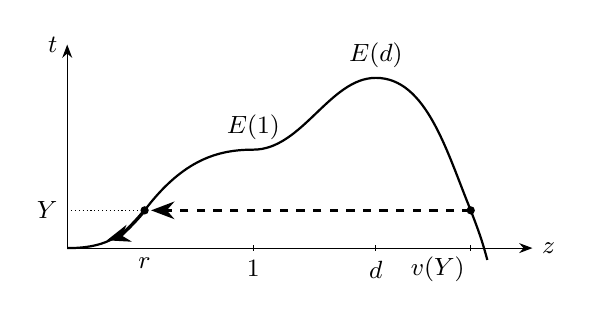
\begin{tikzpicture}[x=1.17cm,y=0.94cm,>=Stealth,font=\small]
\draw[->] (0,0)--(5.05,0) node[right] {$z$};
\draw[->] (0,0)--(0,2.75) node[left] {$t$};
\draw[thick] (0,0) .. controls (.38,0) and (.59,.12) .. (.84,.51)
 .. controls (1.26,1.2) and (1.64,1.33) .. (2.02,1.33)
 .. controls (2.55,1.33) and (2.85,2.3) .. (3.35,2.3)
 .. controls (3.9,2.3) and (4.12,1.30) .. (4.38,.51)
 .. controls (4.46,.25) and (4.5,.12) .. (4.56,-.16);
\draw[densely dotted] (0,.51) node[left] {$Y$}--(.84,.51);
\draw[very thick,dashed,->] (4.38,.51)--(.91,.51);
\draw[very thick,->] (.84,.51) .. controls (.72,.32) and (.57,.16) .. (.43,.105);
\fill (.84,.51) circle (1.5pt) (4.38,.51) circle (1.5pt);
\draw (2.02,.04)--(2.02,-.04) node[below] {$1$};
\draw (3.35,.04)--(3.35,-.04) node[below] {$d$};
\node[below] at (.84,0) {$r$}; \draw (4.38,.04)--(4.38,-.04) node[below left,inner sep=2pt] {$v(Y)$};
\node[above] at (3.35,2.3) {$E(d)$}; \node[above] at (2.02,1.33) {$E(1)$};
\end{tikzpicture}
\caption{Turning launch at $Y=E(r)$, shown on the limiting even profile
(schematic). In forward time in the reflected right half-plane the
trajectory leaves the falling root $v(Y)>d$, moves inward to the rising
root $r<1$ at this limiting height, and follows the inner branch toward
the axis. The backward half (omitted) follows the falling branch in
increasing $t$ and reaches the upper axis through the distant maximum.}\label{fig:turning-supp}
\end{figure}

At~\eqref{eq:deg12-3matches}, the last inflection sign ($+$) and the first section-entrance sign ($-$) frame the matched inner reference $\D(ST)=0$. If we detune $a$ upward so that $\D(SH_*)<0$ (sign $-$ after the $+$ from $t=-1/2$), then $\D(ST)$ also becomes negative. The first section-entrance sign is also negative. Two more brackets
therefore require a positive sign between $ST$ and $S h_+(4/5)$. A regular turning orbit on the outer falling branch supplies that positive bridge.

For a small fixed $r\in(0,1/2)$, put $Y=E(r)\in(0,E(1))$ and, on each side $s\in\{\pm 1\}$ at a match of~\eqref{eq:deg12-3matches}, launch an orbit at its outer turning point $(z,t)=(v_s(Y),Y)$ where $\Phi_s(v_s(Y))=Y$ on the falling branch ($v_s(Y)>d$). Denote its backward scaled upper hit by $H_s(Y)$ and its forward physical lower-axis hit magnitude by $b_s(Y)$. Let $I_e(Y)=\int_{C_0/L}^{r_e(Y)}\Phi_{\mathrm{ev}}'(z)^2\,\dd z/z$ be the rising action in the $z$ coordinate, ending at the regular inner root $\Phi_{\mathrm{ev}}(r_e(Y))=Y$ near $r$. Uniformly for levels in a small neighborhood of $Y$, we claim that $H_s(Y)<H_*$, $b_s(Y)>w_*$, and
\begin{align}
  \eps\log\big(H_* - H_s(Y)\big) &= -J_e(Y) - s\eta V(Y) + O_r(\eta^{3/2}),\label{eq:turn-back}\\
  \eps\log\big(b_s(Y) - w_*\big)  &= -I_e(Y) - s\eta W(r) + O_r(\eta^{3/2}).\label{eq:turn-fwd}
\end{align}

To prove~\eqref{eq:turn-back}, run~\eqref{eq:scalar-u} in backward time ($t$ increasing). The outer reference $u_{\mathrm{ref}}^{\mathrm{out}}(t)$ from $(u,t)=(0,-1)$ tracks the falling root $u_s(t)=v_s(t)^2/2$ from lower heights ($t<Y$) while remaining strictly \emph{above} $u_s(t)$ in $u$ (to the right of the falling graph in $(z,t)$): indeed, $e(t)=u_{\mathrm{ref}}^{\mathrm{out}}(t)-u_s(t)>0$ satisfies $e'(t)=[\phi_s]_{u_{\mathrm{ref}}^{\mathrm{out}},u_s}\,e(t)/\eps - u_s'(t)$, where both $-[\phi_s]_{u_{\mathrm{ref}}^{\mathrm{out}},u_s}$ and $-u_s'(t)$ are bounded above and away from zero on a compact regular approach interval $[Y-\delta_r,Y]$. Variation of constants after entry into the falling-branch tube therefore places $e(Y)=u_{\mathrm{ref}}^{\mathrm{out}}(Y)-u_s(Y)$ strictly between $c_r\eps$ and $C_r\eps$ ($0<c_r<C_r$). Since the turning orbit starts at $u_{\mathrm{turn}}(Y)=u_s(Y)<u_{\mathrm{ref}}^{\mathrm{out}}(Y)$, trajectory order preserves this positive gap to the upper axis ($H_s(Y)<H_s^*=H_*$), and since $\eps|\log\eps|=O(\eta^{10}|\log\eta|)=o(\eta^{3/2})$, applying the upper-hit derivative~\eqref{eq:Ks-deriv} and falling-action expansion of~\eqref{eq:deg12-cap} from $t=Y$ yields~\eqref{eq:turn-back}.

To prove~\eqref{eq:turn-fwd}, follow $u_{\mathrm{turn}}(t)$ and the inner reference $u_{\mathrm{ref}}^{\mathrm{in}}(t)$ from $(0,ST)$ in forward time ($t$ decreasing from $Y$). Because $Y=E(r)<E(1)$ lies strictly below the stationary inflection and $T>E(1)>Y$, at the launching ordinate $t=Y$ the inner reference is already tracking the inner rising root $\tilde u_s(t)=r_{s,\eta}(t)^2/2$ near $r^2/2$, whereas $u_{\mathrm{turn}}(Y)=u_s(Y)=v_s(Y)^2/2$ starts near $v(Y)^2/2>d^2/2>r^2/2$. Thus, \emph{at the launching ordinate $t=Y$ itself}, $u_{\mathrm{turn}}(Y)-u_{\mathrm{ref}}^{\mathrm{in}}(Y)=\frac12(v(Y)^2-r^2)+o(1)\ge c_r'>0$ is bounded above and away from zero; trajectory order preserves $u_{\mathrm{turn}}(t)>u_{\mathrm{ref}}^{\mathrm{in}}(t)$ down to $\Sigma_-$, proving $b_s(Y)>w_s(ST)=w_*$ and bounding the initial term $\eps\log\big(u_{\mathrm{turn}}(Y)-u_{\mathrm{ref}}^{\mathrm{in}}(Y)\big)=O_r(\eps)$ in~\eqref{eq:secant-exact}. Next, since $\Phi_s(z)>Y$ across the open interval $(r_{s,\eta}(Y),v_s(Y))$, fix $\nu_r>0$ small so that $-\phi_s'\ge 2c_r>0$ and $-u_s'\ge 2c_r>0$ on $[u_s(t)-\nu_r,u_s(t)]$, $\phi_s'\ge c_r''>0$ and $|\tilde u_s'|\le C_r''$ on $[\tilde u_s(t),\tilde u_s(t)+\nu_r]$, and $\phi_s\ge Y+\kappa_r$ ($\kappa_r>0$) across $[\tilde u_s(Y)+\nu_r,u_s(Y)-\nu_r]$:
\begin{enumerate}
  \item[\textup{1.}] \emph{Falling-root escape:} while $\tilde e(t):=u_s(t)-u_{\mathrm{turn}}(t)\in[0,\nu_r]$, $\dd\tilde e/\dd(-t)=-u_s'(t)-[\phi_s]_{u_{\mathrm{turn}},u_s}\tilde e/\eps\ge c_r+c_r\tilde e/\eps$ from $\tilde e(Y)=0$, reaching $\tilde e=\nu_r$ in height descent $\tau_1\le(\eps/c_r)\log(1+\nu_r/\eps)=O_r(\eps|\log\eps|)$;
  \item[\textup{2.}] \emph{Horizontal bridge:} across $[\tilde u_s(Y)+\nu_r,u_s(Y)-\nu_r]$, $\dd u_{\mathrm{turn}}/\dd(-t)=(t-\phi_s(u_{\mathrm{turn}}))/\eps\le -\tfrac12\kappa_r/\eps$, taking height descent $\tau_2=O_r(\eps)$;
  \item[\textup{3.}] \emph{Inner rising-root capture:} on $[\tilde u_s(t),\tilde u_s(t)+\nu_r]$, $q(t):=u_{\mathrm{turn}}(t)-\tilde u_s(t)>0$ obeys $\dd q/\dd(-t)\le C_r''-c_r'' q/\eps$, entering an $O_r(\eps)$ neighborhood (and hence the $\eta^{7/2}$-tube of Proposition~\ref{prop:moving-layer}) within $\tau_3=O_r(\eps|\log\eps|)$ height descent.
\end{enumerate}
Throughout the entire transfer interval $[Y-(\tau_1+\tau_2+\tau_3),Y]$ of height length $O_r(\eps|\log\eps|)$, both $u_{\mathrm{turn}}$ and $u_{\mathrm{ref}}^{\mathrm{in}}$ remain inside the compact positive interval $[\frac14 r^2,v(0)^2]$ where $\phi_s'$ and $[\phi_s]_{u_{\mathrm{turn}},u_{\mathrm{ref}}^{\mathrm{in}}}$ are $O_r(1)$, so~\eqref{eq:secant-exact} changes by $O_r(\eps|\log\eps|)=o(\eta^{3/2})$. Below $Y-(\tau_1+\tau_2+\tau_3)$, Proposition~\ref{prop:moving-layer} applies with \emph{no} intervening fold on $[C_0/L,r_{s,\eta}(Y)]$ (all compact seed critical points lie below $z=C_0/L$ at height $O(\eta^6)\ll\eta^3$), giving $\eps\log(b_s(Y)-w_*)=-\int_{C_0/L}^{r_{s,\eta}(Y)}\Phi_s'(z)^2\,\dd z/z+O_r(\eta^3)$. Expanding the upper integration limit $r_{s,\eta}(Y)=r_e(Y)-s\eta B(r)/E'(r)+O_r(\eta^{3/2})$ contributes the moving-endpoint term
\[
  \big(r_{s,\eta}(Y)-r_e(Y)\big)\frac{E'(r)^2}{r} + O_r(\eta^{3/2}) = -s\eta\,A(r)B(r) + O_r(\eta^{3/2}),
\]
which combines with the cross term $2s\eta\int_0^r A(z)B'(z)\,\dd z+O_r(\eta^{3/2})$ (the $[0,C_0/L]$ cutoff costing $O(\eta^{10})$ and $(\Phi_{\mathrm{od}}')^2/z$ costing $O_r(\eta^2)$) to give $s\eta W(r)=-s\eta I_1(r)$ in the positive rising action.
It enters~\eqref{eq:turn-fwd} with the opposite sign.

Because an earlier falling-branch trajectory already lies strictly to the right when a later turning orbit launches, $H_s(Y)$ decreases strictly with $Y$. At $Y=E(r)$, differentiating the actions at their regular spatial endpoints gives
\[
 J_e'(Y)=\frac{\Phi_{\mathrm{ev}}'(v_e(Y))}{v_e(Y)}
        =A(v(Y))+O_r(\eta)<0,\qquad
 I_e'(Y)=\frac{\Phi_{\mathrm{ev}}'(r_e(Y))}{r_e(Y)}
        =A(r)+O_r(\eta).
\]
The first derivative stays negative near $Y$, so~\eqref{eq:turn-back}
brackets a unique $Y_-=Y+O_r(\eta)$ with $H_-(Y_-)=H_+(Y)$.
Expanding~\eqref{eq:turn-back} and then subtracting~\eqref{eq:turn-fwd} yields
\begin{align}
  Y_- - Y &= 2\eta\,\frac{V(Y)}{A(v(Y))} + O_r(\eta^{3/2}),\label{eq:shift-turn}\\
  \eps\log\frac{b_+(Y)-w_*}{b_-(Y_-)-w_*} &= -2\eta\!\left(W(r) - \frac{A(r)V(Y)}{A(v(Y))}\right) + O_r(\eta^{3/2}).\label{eq:bridge}
\end{align}
On the compact limiting match set $\{\theta=0,\ V(0)=0,\ d\in D\}$, $-A(v(0))$ and $\beta$ have positive minima, and as $r\downarrow 0$ we have $A(r)=r^4+O(r^6)$ and $B(r)=-\beta r^5+O(r^7)\implies W(r)=-\frac19\beta r^9+O(r^{11})$, while smoothness of the regular falling root $v(\cdot)$ near $0$ with $V(0)=0$ gives $V(E(r))=O(E(r))=O(r^6)$ and hence $A(r)V(E(r))/A(v(E(r)))=O(r^{10})$. Fixing $r>0$ sufficiently small first (before choosing $\eta>0$ small) makes $W(r)-A(r)V(Y)/A(v(Y))<0$ uniformly near the limiting match set, so~\eqref{eq:bridge} gives $b_+(Y)>b_-(Y_-)$, i.e., $\D(SH_+(Y))>0$.

\begin{remark}[Explicit rational turning radius]\label{rem:rational-turn}
At $\theta=0$ on the narrowed rational interval $D'=[1.19888999543,\,1.19888999544]\subset D$, $V(0)$ already has opposite strict signs at the two endpoints, and at the explicit rational radius $r=1/4$, monotone interval arithmetic certifies $\beta^{-1}\big(W(1/4)-A(1/4)V(E(1/4))/A(v(E(1/4)))\big)\in(-3.1\cdot 10^{-7},-2.8\cdot 10^{-7})<0$ uniformly across all $d\in D'$. The strict face and bridge inequalities persist at finite matches with $\theta_\eta\to0$ when the matching rectangle uses $D'$.
\end{remark}

\begin{proof}[Completion of the proof of Theorem~\ref{thm:deg12}]
Fix a sufficiently small $\eta>0$ and a matched solution $(d_\eta,\theta_\eta)$ of~\eqref{eq:deg12-3matches} with $a_*=a_\eta(d_\eta,\theta_\eta)\in\operatorname{int}J$, and put $h_{\mathrm{dir}}=H_*-g_-^b$. Consider the $20$ physical upper heights $(H_1,\dots,H_{20})$ defined by
\[
  \big(h_0,\dots,h_4,\ St_0,\dots,St_7,\ ST(d_\eta),\ SH_+(Y),\ S h_+(4/5),\ S h_+(0),\ S h_+(-20),\ Sh_{\mathrm{dir}},\ SH_*\big).
\]
The compact heights end at $h_4=4.36$, while
$St_0=S(E(1)+o(1))\to\infty$. Since $K>0$, the order of the eight
$St_i$ is the order of the cubic samples $\xi_i$. The next two
inequalities follow from
$T(d_\eta)-t_7=(E(d_\eta)-E(1))/2+o(1)>0$
and $H_+(Y)=E(d_\eta)+o(1)>T(d_\eta)$.
For the remaining heights,
$d_\eta<v(Y)<v(0)<v(-1/2)$ gives
$0<J_o(Y)<J_o(0)<J_o(-1/2)$. The absolute actions
in~\eqref{eq:deg12-cap} and~\eqref{eq:turn-back} separate the turning,
entrance and direct heights. Within the entrance list,
$-A(v(0))>0$ in~\eqref{eq:deg12-fine} orders the three gaps. Together,
\[
 H_*-H_+(Y)\gg g_+(4/5)>g_+(0)>g_+(-20)\gg g_-^b>0 .
\]
This orders all twenty heights. At $a=a_*$ their mismatches are
\[
\begin{array}{c|ccccccc}
k&1\text{--}5&6\text{--}13&14&15&16\text{--}18&19&20\\ \hline
\sgn\D(H_k,a_*)&{+}{-}{+}{-}{+}&{-}{+}{-}{+}{-}{+}{-}{+}&0&+&{-}{+}{-}&+&0 .
\end{array}
\]
Now hold $(d_\eta,\theta_\eta,\eta)$ (hence $a_2,\dots,a_{12}$) and \emph{all twenty physical heights $H_1,\dots,H_{20}$ fixed}, and vary only the linear coefficient $a$ upward on a small open interval $(a_*,a_*+\delta_0)\subset\operatorname{int}J$. Since $|F_{\eta,a_*}'(0)|=|a_*|<2$ and $(0,H_{20})=(0,SH_*)$ has transverse lower-axis hits $(0,-S)$ on both sides, Lemma~\ref{lem:half-returns}(iii) gives smooth transverse half-returns $w_\pm(h,a)$ with $w_\pm'>0$ across all of $(0,H_{20}]$ for $|a-a_*|<\delta_0$. By Lemma~\ref{lem:rotational}, $\partial_a\D(h,a)<0$, so for every $a\in(a_*,a_*+\delta_0)$ both zeros at $H_{14}=ST(d_\eta)$ and $H_{20}=SH_*$ become strictly negative while all $18$ nonzero strict signs persist, yielding $20$ strictly alternating signs $+,-,+,-,\dots,+,-$ and $19$ pairwise disjoint open brackets $(H_{k-1},H_k)$ for $2\le k\le20$. Applying Proposition~\ref{prop:sard}(i) ($\sigma_{\mathrm{det}}=-1$) selects a Sard regular value $a_{\mathrm{reg}}\in(a_*,a_*+\delta_0)$ at which every bracket contains a simple zero $r_k$ ($\partial_h\D(r_k,a_{\mathrm{reg}})\neq 0$, multiplier $w_+'(r_k)/w_-'(r_k)\neq 1$), giving $19$ distinct hyperbolic limit cycles on a nonempty open exact-degree-twelve neighborhood containing $\Q^{12}$ points.
\end{proof}

\subsection{An unsplit inner profile in degree nine}\label{subsec:deg9}
\begin{proof}[Completion of Proposition~\ref{prop:low-deg} for $n=9$]
Write $c=a_6>0$, $b=a_5<0$ and fix an outer radius $L>2$. Use
\[
 \begin{aligned}
 A(z)&=6c z^4(1-z^2/L^2),& E(z)&=\int_0^z v A(v)\,\dd v,\\
 B_{\lambda,\theta}(z)&=b z^5(1-z^2/L^2)
     +\lambda L^5(z/L)^7(1-z^2/L^2)+\theta L^5(z/L)^7 .
 \end{aligned}
\]
The maximum of $E$ is at $L$. For $Y<E(L)$ let $v(Y)>L$ be the
falling root and use the same positive-action convention as in
Section~\ref{subsec:deg12-prep}, with $W(r)=\int_0^r(AB'-A'B)\,\dd z$,
$V(Y)=W(v(Y))-W(L)$. Set $z=LZ$. Dividing $A,E,B$ by
$L^4,L^6,L^5$ gives the profiles of Proposition~\ref{prop:cap-transfer}
for $m=6,j=5$, with $v(0)/L=\sqrt{4/3}$. At $\theta=0$ the
normalized density of $V$ has the sign of $b+3\lambda Z^2$ on
$Z>1$. Its integral at $Y=0$ is affine in $\lambda$, with positive
slope and negative value at $\lambda=0$. Thus $V_{\lambda_0,0}(0)=0$
at a unique $\lambda_0>0$, independent of $L$. A bounded $Y$ displaces
the normalized root by $O(|Y|L^{-6})$. Since $V$ scales as $L^9$ and
$|A(v(Y))|\asymp L^4$, we have
$|V_{\lambda_0,0}(Y)/A(v(Y))|\le C|Y|/L$.

On the inner branch take $r=1$, $Y=E(1)$. As $L\to\infty$,
$W(1)=\frac23 cb+O(L^{-2})$ and
$W(1)-A(1)V(Y)/A(v(Y))=\frac23 cb+O(L^{-1})$ at this calibration.
Fix $L$ large enough that both are strictly negative.
Choose $T=(Y+E(L))/2$ and a section $1<z_e<L$ with $E(z_e)>T$.
For $\delta=R^{-1}$, $\eps=\delta^{10}$, set
\[
 F_{R,a}(x)=R^6 E(x/R)+R^5 B_{\lambda,\theta}(x/R)
                  +a_4x^4+a_3x^3+a_2x^2+ax .
\]
This converges to $p_a$ on fixed physical intervals. On $0<z\le z_e$,
$E(z)/z^6$ has positive infimum and $z|B(z)|/E(z)$ is bounded
uniformly for bounded parameters. These bounds give $F_{R,a}(sx)\ge c_1x^6$
on $X\le x\le Rz_e$ after $X$ and then $R$ are large.
The wall at $Rz_e$ traps the upper reference $R^6T$.
Capture at $y=8$ and the two faces in Lemma~\ref{lem:seed} close that
reference at a unique continuous $a_R(\lambda,\theta)\in\operatorname{int}J$,
by the strict derivative~\eqref{eq:rot-half}.

With $L$ fixed, the coarse and fine falling-branch estimates
(3.15) and (3.17) of the main paper apply in the $R$ scaling.
Indeed the scaled even remainder is $O(\delta^2)$, the odd remainder
after $\delta B$ is $O(\delta^3)$ on fixed intervals, and
$\eps|\log\eps|=o(\delta^6)$. The peak splitting has coefficient
$B(L)=\theta L^5$, and $\partial_\lambda V(0)>0$.
Consequently the two residuals have opposite signs on the respective
faces of $[\lambda_0-\rho_0,\lambda_0+\rho_0]\times
[-\sqrt\delta,\sqrt\delta]$, with $0<\rho_0<\lambda_0/2$ fixed.
The rectangle argument of Proposition~\ref{prop:cap-transfer} gives
$H_+^*=H_-^*=H_*$ and $g_+(\delta^6\Delta)=g_-(0)$ for
$\Delta=3/500$, at $\theta_R=O(\delta)$ and
$\lambda_R=\lambda_0+O(\delta)>0$. In particular
$[x^9]F_{R,a}=-\lambda_R R^{-4}L^{-4}<0$, and every higher power vanishes.

The upper mismatch $\D(R^6Y)$ has sign $W(1)<0$ by the regular rising-root
calculation of Section~\ref{sec:deg12}. For the turning launch at
$(v_s(Y),Y)$, equality of the backward upper hits shifts the minus
level by $2\delta V(Y)/A(v(Y))+O(\delta^2)$.
The proof of~\eqref{eq:bridge} applies at these regular roots: the
forward passage has no folds before $r=1$, the backward passage has one
outer maximum, and the same two matched references bound both gaps.
The resulting mismatch has sign
$-\sgn(W(1)-A(1)V(Y)/A(v(Y)))=+$. Thus the samples at $R^6Y$ and
$R^6H_+(Y)$ give successive negative and positive signs. The latter
height exceeds $R^6T$ since $H_+(Y)\to E(L)>T$.
Since $J_o(Y)<J_o(0)$, all three paired section heights are higher
still and below $R^6H_*$. They occur in the order $4/5,0,-20$ by the positive slope in (3.17) of the main paper. The uniform bound $F_{R,a}(sx)\ge c_1x^6$
on $[X,Rz_e]$ gives a tail error $O(X^{-4})$ and transfers all three
strict signs of Lemma~\ref{lem:seed-incoming}. The five compact
signs persist by compact convergence. Holding all eleven upper
heights fixed gives in increasing order
\[
  (+,-,+,-,+),\quad -,\quad +,\quad (-,+,-),\quad 0 .
\]
The final zero is the upper hit from the common lower point $(0,-R^6)$.
Decrease $a$ slightly in $J$ to make it positive and apply
Proposition~\ref{prop:sard}(i) on the trapped return interval.
The ten brackets give ten simultaneous hyperbolic cycles on an open
set of exact degree nine.
\end{proof}

\begin{remark}[Degree-twelve ansatz constraints]\label{rem:deg12-obstruction}
Within the ansatz of Section~\ref{subsec:deg12-prep} ($A$ as in~\eqref{eq:deg12-even} and $B$ odd with quintic germ satisfying $B(1)=B(d)=0$), any polynomial $B$ of degree at most $9$ is a scalar multiple of $z^5(1-z^2)(1-z^2/d^2)$, whose Wronskian with $A$ equals a nonzero multiple of $\omega(z)(1+z^2)$ and therefore cannot satisfy $\M(B)=0$; degree $11$ in $B$ is minimal for that ansatz. Likewise, Lemma~\ref{lem:deg12-radius} gives $V(E(1))>0$ at every limiting match, so~\eqref{eq:shift-turn} shifts the cross-side turning height near $E(1)$ by $O(\eta)$, strictly larger than the $O(\eta^{3/2})$ width of the split cubic windows, preventing direct transfer of the four incoming cubic changes inside this joint degree-twelve family.
\end{remark}


\appendix
\renewcommand{\thesection}{S\Alph{section}}
\section{An explicit weak-damping field}\label{sec:weak}
For a primitive $F(x)=\sum a_jx^j$ define $d=\lfloor(n-1)/2\rfloor$
and $\Pi_F(h)$ as the first return height. The weak-domain estimate used
here is Theorem~A.1 of the main paper. With
\begin{equation}\label{eq:weak-defs}
  \sigma_a(h)=\sum_{j=1}^n |a_j|h^{j-1},\quad
  \rho=2^{-(n+6)},\quad
  L_d=(d+1)!(d+1)2^d,\quad
  \delta_n=\frac{\rho^2}{72(n+2)d!\,L_d\,n^{d(d+1)/2}},
\end{equation}
a nonzero odd part permits at most $d$ positive return zeros on
$\sigma_a(h)\le\delta_n$, counted with multiplicity. Set
$c_k=4^{-(k+1)}\binom{2k+2}{k+1}$ and
$\kappa_n=\delta_n n!/[2^{n-1}(4n)^n]$.
For $q(u)=\prod_{i=1}^d(u-h_i^2)=\sum_{k=0}^dq_k u^k$ the realizing
polynomial and the uniform remainder are
\begin{equation}\label{eq:weak-realize}
  F_\eps(x) = \eps x^{2\lfloor n/2\rfloor} + \eps^\ell\sum_{k=0}^d \frac{q_k}{c_k}\,x^{2k+1}\qquad (\eps>0).
\end{equation}
\begin{equation}\label{eq:weak-cauchy-err}
  \left|\frac{\Pi_{F_\eps}(h)-h}{h\eps^\ell} + 2\pi q(h^2)\right| \le \frac{4\,\sigma_{F_\eps}(h)}{\rho^2}\sum_{k=0}^d\left|\frac{q_k}{c_k}\right|h^{2k} = O(\eps)\qquad (0<h\le 1).
\end{equation}
The estimate holds when $\sigma_{F_\eps}(1)\le\delta_n$.
\begin{remark}[Fully specified rational witness at $n=12$]\label{rem:fixed-weak-witness}
Setting $n=12$ ($d=5$), $\ell=5$, $\eps=\tau=10^{-60}$, and $h_i=i/6$ ($1\le i\le 5$) in~\eqref{eq:weak-realize} specifies an explicit rational polynomial $F_\tau(x)=10^{-60}x^{12}+10^{-300}\sum_{k=0}^5(q_k/c_k)x^{2k+1}$ of exact degree twelve whose odd perturbation vanishes through fourth order in $\tau$. Direct rational evaluation (verified in \texttt{checks/\allowbreak verify\_\allowbreak weak\_\allowbreak return.py}) gives $\sigma_{F_\tau}(1)<\delta_{12}$, where $1/\delta_{12}=\allowbreak 17{,}704{,}107{,}497{,}153{,}401{,}118{,}\allowbreak 612{,}992{,}587{,}674{,}419{,}200$, and $\sup_{|x|\le 2}|F_\tau'(x)|\le\sum_{j=1}^{12}j|a_j|2^{j-1}<\kappa_{12}$. At the ten rational endpoints $h_{i,\pm}=(4i\pm 1)/24$ ($1\le i\le 5$), the Cauchy remainder~\eqref{eq:weak-cauchy-err} is strictly below $4\cdot 10^{-49}$ (and an independent real variational enclosure along $s\in[0,1]$ in the clockwise polar equation of the main paper, Appendix~A is below $2\cdot 10^{-50}$), whereas $6|q(h_{i,\pm}^2)|>3\cdot 10^{-4}$; since $6<2\pi<8$, $(\Pi_{F_\tau}(h)-h)/(h\tau^5)$ has certified endpoint signs $(+,-),(-,+),(+,-),(-,+),(+,-)$. Thus the five disjoint brackets in $(0,1]$ each contain a return zero. They lie in the weak domain since $\sigma_{F_\tau}$ is nondecreasing and $\sigma_{F_\tau}(1)<\delta_{12}$. The odd part is nonzero, so Theorem~A.1(ii) of~\cite{MainArticle} bounds the total multiplicity in that domain by five. Each zero is therefore simple. These five hyperbolic cycles (three attracting and two repelling) account for all cycles with upper heights in $\sigma_{F_\tau}(h)\le\delta_{12}$.

\end{remark}


\section{A fixed rational field and its finite certificates}\label{app:repro}

\begin{proposition}[Six cycles at specified coefficients]\label{prop:fixed-six}
In~\eqref{eq:deg12-poly} set $d=6/5$, $\sqrt\eta=10^{-40}$,
$\theta=-10^{-20}$ and $a=(a_-+a_+)/2$ with $a_\pm$ from~\eqref{eq:seed-coeffs}.
The resulting rational primitive has degree twelve. Its field has a
hyperbolic cycle in each bracket of Table~\ref{tab:fixed-six} and a
repelling hyperbolic cycle above those five.
\end{proposition}

For a forward arc of the reflected field with $G_s(x)=F(sx)$, let
$\Lambda_s(h)=\int G_s'(x(\tau))\,\dd\tau$ from launch $(0,h)$ to
its first lower-axis hit $(0,-w_s(h))$. This is the negative of the
integrated divergence on that half-arc.

\begin{table}[htbp]
\centering\small
\caption{Physical upper-axis brackets for the fixed negative-tilt field.
Every decimal endpoint is rational. The last column encloses the
integral difference over the whole closed bracket.}\label{tab:fixed-six}
\begin{tabular}{@{}rrrrc@{}}
\toprule
$h_l$ & $h_r$ & $\sgn\D(h_l)$ & $\sgn\D(h_r)$ & $10^5(\Lambda_+-\Lambda_-)$\\
\midrule
3.494474846805 & 3.494474846808 & $+$ & $-$ & $(235,236)$\\
3.848603188665 & 3.848603188668 & $-$ & $+$ & $(-4.1,-3.6)$\\
3.978624148391 & 3.978624148394 & $+$ & $-$ & $(1.5,2.1)$\\
4.324131925377 & 4.324131925381 & $-$ & $+$ & $(-1.5,-0.9)$\\
4.454460589336 & 4.454460589341 & $+$ & $-$ & $(1.8,2.6)$\\
\bottomrule
\end{tabular}
\end{table}


\begin{proof}
Liouville's formula with the normal velocities at the two sections
gives $w_s'(h)=(h/w_s(h))e^{-\Lambda_s(h)}$. At a zero of
$\D=w_+-w_-$ the full multiplier is therefore
$e^{-(\Lambda_+-\Lambda_-)}$.

\emph{Compact brackets.}
Let $Q_s$ be the sextic from~\eqref{eq:seed-coeffs} at the same midpoint,
reflected on side $s$. Summing the absolute differences of the
coefficients weighted by $3^j$, first for $G_s-Q_s$ and then for its
derivative, gives a bound $\delta=2\cdot10^{-74}$ for each on $|x|\le3$.
The leading coefficient of the full primitive is negative.
For each rational endpoint and for each entire height bracket we use
the order-36 dyadic paths of Lemma~\ref{lem:seed}. In normalized time
$0\le v\le1$ let $R$ bound the residual against the sextic vector
field multiplied by the physical step $b$ (the residual is the path
derivative minus $b$ times that field). Its polynomial coefficients
through degree 216 are formed exactly on rational data. Round path
coefficients to the $2^{-256}$ grid and error bounds outwards.
The symmetric part of the sextic Jacobian is
$\operatorname{diag}(-Q_s',0)$. The completed squares of
Lemma~\ref{lem:seed} give logarithmic norm at most $\gamma=1$ for
$x\ge-1/100$, and at most $1/250$ for $x\ge0$. Thus a valid radius is
\[
 e_{\rm out}=\frac{e_{\rm in}+R+b\delta}{1-b\gamma}.
\]
Indeed $e'\le b\gamma e+R+b\delta$ until first exit.
Each accepted tube lies inside its domain; the smaller $\gamma$ is
used only after verification of positivity with the wider tube.
Centering the initial tube at the bracket midpoint with radius half
its width covers every launch therein.

Compose $Q_s'$ with the proposed $x(v)$, integrate its polynomial
on each step, and enclose the coefficients by outward dyadic rounding.
The additional radius in the integral is at most
$b(\|Q_s''\|e_{\rm out}+\delta)$. The departure and intermediate
tubes have $x>0$ after the initial crossing. On the final step the
enclosed arc crosses $x=0$ with $-\dot x\ge v_0>0$. At the proposed
event time found by bisection the true time differs by at most
$(|x_{\rm app}|+e_{\rm out})/v_0$ in physical units. Multiply this
bound by $\sup|G_s'|$ for the last integral and by $\sup|x|$ for the
hit ordinate, in addition to the path error there. The resulting endpoint
signs and full-interval integral differences are in Table~\ref{tab:fixed-six}.
Order and continuity give a zero in each interval and the displayed
multiplier formula proves simplicity.

\emph{Outer section hits at the fixed scale.}
Set $P_s(z)=F(sLz)/S$, $u=z^2/2$, $p_s(u)=P_s(\sqrt{2u})$,
$t=y/S$, $\eps=L^2/S^2$, and put
$\lambda=\sqrt\eta$, $K=10^7$, $c=10^{-4}$, $\rho=\lambda^4$, $\nu=\rho^2$.
The rational profile bounds needed below are as follows. The maximum
$M_s$ on $0\le u\le2$ occurs at $1.18<z_m<1.22$,
$0.012<M_s<0.014$, and
\[
 P_s(d)\le M_s\le P_s(d)+m_{\rm lift},\qquad
 m_{\rm lift}=(10^5\eta)^2/(2\cdot0.1).
\]
On $1.18\le z\le1.22$ one has $p_s''<-0.1$ with opposite signs of
$p_s'$ at the ends; on $1.22\le z\le2$ one has $p_s'<-0.01$,
$P_s(1.22)>0.01$, $P_s(2)<-2$. Further,
$P_s>10^{-3}$ on $[1/2,1.22]$, $P_s<M_s-2c$ on $[0,1.11]$,
$|p_s'|,|p_s''|<K$ on $1/2\le z\le2$, and
$\int_0^{1.10}|P_s'|\,\dd z<2K$. These are finite polynomial
comparisons. Use $p_s'=P_s'/z$, $p_s''=(zP_s''-P_s')/z^3$ away
from zero. For a polynomial $Q(a+(b-a)v)=\sum_j c_j v^j$ of
degree $k$, its Bernstein coefficients
$\sum_{j\le i}\binom{i}{j}c_j/\binom{k}{j}$ bound it on $0\le v\le1$.
The explicit even profile increases up to $d$; coefficient norms
bound its perturbation, yielding the stated height margins below
$z=1.18$. At $d$, $|p_s'(d^2/2)|\le10^5\eta$ and the curvature
bound yields the lift. Translating $P_+(z)+10^{-3}z^{12}$ by $2$
gives negative coefficients, proving the tail bound for $z\ge2$.

On the plus side follow a launch from $(z,t)=(1/2,y/S)$,
$-1\le y\le9$, backward in physical time. Then $t$ increases and
$\eps u_t=p_+(u)-t$. The falling root $U(t)$ satisfies $|U'|\le1/\rho$
up to $t=M_+-\rho$. Indeed its distance in $u$ from the maximum exceeds
$20\rho$ there, since $200K\rho^2<\rho$. The curvature and outer
slope bounds give $-p_+'\ge\rho$ on $[U(t)-\nu,2]$.
The tube $|u-U(t)|\le\nu$ is invariant. Its boundary speed toward the
root is at least $\rho\nu/\eps$. At launch the orbit is left of
the tube. The bounds through $z=1.22$ and monotonicity thereafter
give at least this speed until capture. Even allowing for the root
speed, it covers distance $2$ within a height increase $\rho$ since
$\eps<\rho^4/8$; the walls at $z=1/2$ and $u=2$ confine this
initial passage. At $M_+-\rho$ the orbit is still away from the axis.
From $t=M_++\rho$ onward it moves inward at speed at least
$\rho/\eps$ and reaches the axis within $2\eps/\rho<\rho$
if it has not already crossed. Boundedness and positive height near
exit exclude an asymptotic stop. Write $\widehat h_+(y/S)$ for this
scaled upper hit. Near exit, from $z=1.10$ to $0$, the inverse equation
$\dd t/\dd u=-\eps/(t-p_+(u))$ has denominator $>c$.

Order gives two physical heights
$H_1=S\widehat h_+(9/S)<H_2=S\widehat h_+(-1/S)$: the earlier
launch lies to the right of the section when the later one starts.
Both are strictly inside the rational enclosure
\[
 \mathcal I=\big(S(P_+(d)-\rho),\ S(P_+(d)+m_{\rm lift}+2\rho)\big).
\]
Its lower endpoint exceeds $4.6$. At the rational upper endpoint
$t\ge M_++2\rho$ initially. In forward time $\eps\,\dd u/\dd(-t)=t-p_+$,
so the loss in height to $u=2$ is at most $2\eps/\rho<\rho$.
From there the tail bound gives at most
$\eps\int_2^\infty[10^{-3}(2u)^6]^{-1}\dd u=25\eps/256<\rho$
before escape at positive height. The sign tests use $H_1,H_2$.

\emph{Signs at the two hits.}
The rational comparison $SP_-(d)>\sup\mathcal I$ makes $x=Ld$ a
forward wall on the minus side. On both sides $G_s(x)>8x^6$ for
$2\le x\le L/2$ and $G_s(x)>x^6/100$ on $L/2\le x\le Ld$.
For these tests use the sextic coefficient error on $[2,10]$ with
weights $10^j$, the factorization of $E'$ in~\eqref{eq:deg12-even}
from $10$ to $L/2$, and $P_s>10^{-3}$ thereafter.
At $8\le y\le9$, $v=x^2/2$ obeys $\dd v/\dd(-y)=y-G_s(x)$.
For $v\ge50$ this is at most $-v^3/25$; for $2\le v\le50$ it is
at most $-4v^3$. The descent needed to reach $x\le2$ is less than
$25/(2\cdot50^2)+1/32<1$. The boundary at $x=2$ points inward
throughout this range. Thus at $y=8$ the minus arc, as well as the
plus arc through $(L/2,9)$, lies in $0\le x\le2$. The wall at $x=3$
and the focus condition $|a|<2$ give compact returns. For their hit
magnitudes $B_s(q,8)$ from $(q,8)$ the compact tubes above give
\[
 B_+(2,8)-B_-(0,8)<-2\cdot10^{-32},\qquad
 0.03<B_-(0,8)\le B_-(2,8)<0.1.
\]
Monotonicity in $q$ yields $\D(H_1)<0$. From $(L/2,-1)$ the plus
arc moves inward to $x=2$ by the same tail bounds and returns inside
the compact wall with magnitude $>1$. Hence $\D(H_2)>0$. Order
and the bounding returns give continuity throughout $[H_1,H_2]$.
Any zero in the internal bracket has common lower magnitude $<0.1$
and plus section ordinate $y\in(-1,9)$.

\emph{Multiplier of the outer zero.}
In scaled coordinates $\eps \Lambda_s=\int p_s'(u)\,|\dd t|$.
On the backward-tracked part of the plus arc the slope is negative;
for $t\in[0.002,0.003]$ it is below $-0.01$ since the tube lies
beyond $z=1.22$. This contributes at most $-10^{-5}$. The entrance
and exit layers above $z=1.10$ cost at most $4K\rho$ in total, and
the final inverse chart costs at most $2K\eps/c$ by the bound
on $\int |P_+'|$. On the forward leg from $L/2$ to $x=2$ one has
$|p_+'|<K$: on $0.01/L\le z\le d$ bound the singular linear
coefficient divided by $z$ using $z\ge0.01/L$, and bound the
remaining polynomial by its coefficient norm. The available physical
height change is less than $9.1$, giving $10K/S$.

On the minus side the initial passage to $x=0.01$ has $t-p_->0.009$
while $t\ge0.01$; the height loss is at most
$\eps(0.01/L)^2/(2\cdot0.009)<0.002$. The inverse chart contributes
at most $2K\eps/0.009$ in absolute value. The boundary at $x=0.01$
points right down to $y=8$. There $z\le d$ by the wall. On this
portion $E'(z)/z\ge0$ and the correction to the slope has magnitude
$<10^{-8}$ using $z\ge0.01/L$. The possible negative contribution
is at most $0.014\cdot10^{-8}$ in magnitude.

For either remaining compact arc, $|G_s'|<10^5$ on $[0,3]$.
Above $x=0.01$ the time is at most $9.1/0.01$. After crossing
inward through $x=0.01$ the monotonicity of $y$ prevents recrossing.
Here $|G_s(x)/x|<0.2$ gives angular velocity at most $-0.9$, so
the remaining time is less than five. Each compact part contributes
less than $10^8\eps$ in absolute value. Substitution of the fixed
scales gives
\begin{align*}
 \eps \Lambda_+ &\le -10^{-5}+4K\rho+2K\eps/c+10K/S+10^8\eps<-9\cdot10^{-6},\\
 \eps \Lambda_- &\ge -2K\eps/0.009-0.014\cdot10^{-8}-10^8\eps>-10^{-6}.
\end{align*}
Thus $\eps(\Lambda_+-\Lambda_-)<-8\cdot10^{-6}$ at every zero in
$(H_1,H_2)$. Its multiplier exceeds one. This bracket and the five
compact brackets are disjoint.
\end{proof}

\subsection*{What the fixed-scale matching tests resolve}
At $\lambda=\sqrt\eta=10^{-40}$ the signs on the parameter faces give
a real solution of the three matching equations. At a match the entrance comparisons
at $4/5,0,-20$ have signs $-,+,-$ and the direct launch gives $+$.
The bounds below give necessary tolerances for mixed shoulder signs
and for paired section hits in the stated windows. The eight shoulder
signs used for nineteen cycles follow from the moving-fold estimate
as $\eta\to0$ in Proposition~\ref{prop:moving-layer}. For the fixed-scale
estimates take the closed parameter box
\[
 1.19888999543\le d\le1.19888999544,\qquad
 |\theta|\le10\lambda,\qquad a_-\le a\le a_+ .
\]
With $\beta=-K/\widehat B'(1)$ as in Section~\ref{subsec:deg12-prep},
the scales $L=-a_5/(6a_6\beta\eta)$, $S=6a_6L^6$ and $\eps=L^2/S^2$
from~\eqref{eq:deg12-poly} give $4.07\cdot10^{-781}<\eps<4.09\cdot10^{-781}$
throughout this box.
Write $H_s^*$ for the scaled upper hit traced backwards from
$(u,t)=(0,-1)$. Let $g_s(r)$ be its positive separation from the
upper hit traced from $(1/8,r)$, and $g_s^b$ its separation from
the hit traced from $(0,-1/2)$.

\emph{The common outer height.}
On either side let $U(t)$ be the falling root of $p_s(U)=t$, let
$z_m$ denote the maximizer and put $v_s(r)=\sqrt{2U(r)}$.
The curvature, wall and tube bounds used in
Proposition~\ref{prop:fixed-six} hold on the whole box by the same
Bernstein and coefficient inequalities. For $-22\le Sr\le1$,
and also for the direct launch with $r=-1/2$, they give
\begin{equation}\label{eq:finite-gap-cost}
 \left|-\eps\log g-
   \int_{z_m}^{v_s(r)}\frac{P_s'(z)^2}{z}\,\dd z\right|<10K\rho .
\end{equation}
Indeed the reference has already reached its tube by the second launch.
The initial $u$-separation lies in $(1/2,2)$. For the positive
separation $b(t)$, $\eps(\log b)'$ equals the secant of $p_s$.
The launch layer costs at most $K\rho$ in the secant integral.
On the common tube the secant differs from $p_s'(U(t))$ by at most
$K\nu$. Omitting the first and last $\rho$ of root tracking costs at most
$2K\rho$. Up to the first inward crossing of $u_c=(1.10)^2/2$ the
remaining layer costs at most $3K\rho$. The secant is bounded there
because at least one $z$ exceeds $1/2$, so $2/(z_1+z_2)\le4$.
Contraction on $[0.002,0.003]$ makes the separation $b_c$ at that
crossing smaller than $2e^{-5\cdot10^{-6}/\eps}$. Both trajectories
then lie below $z=1.11$, with inward speed between $c/\eps$ and
$K/\eps$. Their crossing heights differ by between
$\eps b_c/K$ and $\eps b_c/c$. In the last inverse chart,
the logarithmic derivative of their height difference with respect to $u$
is $\eps/[(t_1-p_s)(t_2-p_s)]\le\eps/c^2$. In $\eps\log$
units this conversion and the initial factor together cost less than
$6000\eps<K\rho$. Finally $t=P_s(z)$ gives the integral in
\eqref{eq:finite-gap-cost}.

For a rational enclosure, bracket $z_m$ by the signs of $P_s'$ on
$[1.18,1.22]$ and the falling root by those of $P_s-r$ on $[1.22,2]$.
Integrate the polynomial part of $P_s'^2/z$ exactly. The remaining
term is $P_s'(0)^2\log(v_s/z_m)$ with $0<\log(v_s/z_m)<1$.
Including the error in~\eqref{eq:finite-gap-cost} gives
$0.0019<-\eps\log g_s(r)<0.0021$ and
$1.3<-\eps\log g_s^b<1.4$. Thus equality of a pair of section
hits in this window forces
\[
 |H_+^*-H_-^*|=|g_+(r_+)-g_-(r_-)|<e^{-4\cdot10^{777}} .
\]
The direct hit is within $e^{-3\cdot10^{780}}$ of its own reference.

\emph{The inner shooting parameter.}
Put $T=(E(1)+E(d))/2$ and fix $d,\theta$. At $a_-,a_+$ respectively
the compact enclosures at $y=8$ give
$\D(ST)>2\cdot10^{-32}$ and $\D(ST)<-6\cdot10^{-32}$, including the
uniform $10^{-72}$ perturbation of the sextic on $[0,3]$ in the
Taylor defect. The linear-parameter sensitivity in
Lemma~\ref{lem:rotational} gives a unique $a_*$ with $\D(ST)=0$.
Consider a shoulder launch from the eight levels in
Proposition~\ref{prop:moving-layer} and the launch at $T$ on the same side.
The shoulder levels lie in $(0.0108,0.0110)$ below $T$.
The wall $z=1.18$ confines both launches. For $0.006\le t\le0.007$,
outside $1/2\le z\le0.9$ the forward equation
$\eps\,\dd u/\dd(-t)=t-p_s(u)$ points toward that strip with magnitude
at least $10^{-4}$ on the right-hand side. Indeed $P_s<0.0019$ below its
left edge and $P_s>0.0071$ above its right edge up to the wall, by
the even profile and its perturbation bound. The distance in $u$ is
less than $2$, so both arcs are inside by $t=0.006$. The boundary
signs persist down to $0.002$, and on the strip $p_s'>0.005$.
On the remaining descent to $y=8$, $z\le0.9$ and $x\ge0.1$ by the
walls. The even slope is nonnegative and the correction exceeds
$-10^{-8}$ there (use $z\ge0.1/L$ in the linear term).
Integrating the secant equation in decreasing $t$ gives a separation
in physical $x^2/2$ below $2L^2e^{-1.9\cdot10^{-5}/\eps}$ at $y=8$.

On this last section the map from $x^2/2$ to the hit magnitude has
derivative $e^{-\Lambda_s}/w_s$ by Liouville's formula, with the
integral and the terminal magnitude now taken from $(x,8)$. For $0\le x\le2$,
order and the endpoint tubes give $0.03<w_s<0.1$. The $x=0$ launch
returns within $41$ time units, allowing $10^{-29}$ for the variation
of the full field over the linear-parameter interval. A larger arc
reaches that terminal ordinate at least as fast, since its $x(y)$ is
larger. Afterwards $\dot x\le-0.03+0.015$ by $G_s'>-0.005$ on
$[0,3]$, so the remaining time is at most $200$. The derivative is
therefore at most $e^{1.25}/0.03<200$. Each shoulder hit lies below
the corresponding reference in magnitude, by order. The two losses
are each less than $400L^2e^{-1.9\cdot10^{-5}/\eps}
<e^{-4\cdot10^{775}}$. Opposite signs at two shoulder heights force
$|\D(ST)|$ below that same bound.

In the formula for $|\partial_a w_s(ST)|$, retain the first
$5\cdot10^{-7}$ time units after $y=8$. There $x\ge0.05$ by
$|\dot x|<10^5$. The remaining compact time is less than $250$ and
$|G_s'|<10^5$. Thus $-\partial_a\D(ST)>e^{-3\cdot10^7}$ throughout
the shooting interval. The mean value theorem gives the necessary
condition
\[
    |a-a_*(d,\theta)|<e^{-3\cdot10^{775}}
\]
for mixed shoulder signs at these fixed $d,\theta$. These estimates
concern the specified box and these choices of sections.

The remaining tests concern the faces of this box and the signs of
individual outer samples. For example, at the two $d$ faces,
\eqref{eq:finite-gap-cost} bounds $(\eps/\eta)\log[g_+(\Delta/S)/g_-(0)]$
in $(-2.974,-2.972)10^{-13}$ and $(4.704,4.707)10^{-13}$, respectively.
At the two $\theta$ faces the peak-lift bound places
$(H_+^*-H_-^*)/\lambda^3$ in $(-46.75,-46.74)$ and $(92.96,92.97)$.
Together with the shooting faces these signs give a real match by the
same box argument as in Section~S5.

After matching, section ordinates require finer control. At $b=0.003$
write $b_s(r)$ for the separation in $u$ from the reference. A section
launch reaches $z=1.22$ within $1500\eps$ in height since
$p_s-t>0.0009$ on the launch segment. Thereafter
$-p_s'\ge0.01$ between that wall and $z=2$, and $|U'|\le100$.
Variation of constants gives distance at most $10002\eps$ from $U$
after $400000\eps$ in height, including the launch layer.
The secant integral then gives
$|\eps\log b_s(r)-\int_r^b p_s'(U(t))\,\dd t|<10^{13}\eps$:
the layer costs at most $2K(400000\eps)$ and the tracked error at
most $10002K\eps$. From $b$ to the inward crossing of $u_c$ the
whole interval stays within width $d_*=2e^{-2\cdot10^{-6}/\eps}$,
using the contraction to $b$ and expansion at most $3K\rho$ in action
thereafter. Its crossing times differ by at most $\eps d_*/c$.
For the map from the section at $b$ to the scaled upper height $H$,
the variational equation gives its derivative as
$(\eps/H)\exp(\eps^{-1}\int_b^H p_s'(u(t))\,\dd t)$.
One can first stop at positive $u$ and then take the limit in the
inverse chart, because $\int_0^{u_c}|p_s'(u)|\,\dd u<2K$ there.
In the common time interval the action difference is at most $Kd_*$,
and in the remaining time interval it is at most $K\eps d_*/c$.
In the inverse chart the height difference contracts. Substituting
$\dd t=-\eps\,\dd u/(t-p_s)$ bounds the difference of the final
actions by $2K\eps^2d_*/c^3$. The transverse prefactor in the
derivative of the upper hit is $\eps/H$, with $H>0.01$, so its
contribution to the oscillation of the scaled log derivative is at most
$100\eps^2d_*/c$. Together these contributions are below $5Kd_*$.
Taking the ratio for two launches now cancels the common terminal
derivative up to this oscillation. With $E(v_0)=0$ on the falling
branch and $c_d=-E'(v_0)/v_0>0.01$, it gives
\[
 \left|S\eps\log\frac{g_s(y_1/S)}{g_s(y_0/S)}
          -c_d(y_1-y_0)\right|<10^{-55},\qquad -25\le y_i\le1 .
\]
Indeed the error from the preceding estimates is below
$3\cdot10^{13}S\eps<10^{-280}$. The slope error over the physical
interval of length $26$ is bounded by
$26(\|R_s'\|+100K(\|R_s\|+25/S))<10^{-55}/2$, with $R_s=P_s-E$
and coefficient norms on $[0,2]$. At a match, tests at
$y-\Delta\pm10^{-12}$ therefore pair each of $4/5,0,-20$ with an
opposite hit. The compact tubes with the $1/448$ tail allowance give
their signs $-,+,-$. For the direct launch one uses the first variation
of the action in~\eqref{eq:finite-gap-cost} along $E+\gamma R_s$.
The peak term vanishes and the falling endpoint supplies
$-(P'/z)R_s$ there. With $\mu=10^7\eta$ bounding $R_s,R_s'$,
the falling root moves at speed at most $100\mu$ in $\gamma$.
Differentiating the integral a second time bounds its interior term
by $2\mu^2$ and the moving-boundary and endpoint terms together by
$(1+500K)\mu^2$. The two Taylor remainders thus cost less than
$10^5K\mu^2$. Including $20K\rho$ from the two gap estimates in the
first-order comparison of Section~S5 gives
$3.8<(\eps/\eta)\log(g_+^b/g_-^b)<5.5$. With common references
the plus direct hit is lower, so the minus direct height has positive
return sign. These tests certify particular comparisons at the fixed
scale. The eight moving-fold signs used together in
Theorem~\ref{thm:deg12} come from the asymptotic estimate of
Proposition~\ref{prop:moving-layer}.

At the two specified midpoints with $d=6/5$ and
$\theta=\pm10^{-20}$, outside the box, the maxima differ already in
height. More precisely $H_+^*-H_-^*$ is in $(6.99,7)10^{-100}$ for
positive tilt and in $(-7,-6.99)10^{-100}$ for negative tilt. These
intervals follow from $P_s(d)\le M_s\le P_s(d)+m_{\rm lift}$ and
$M_s-\rho<H_s^*<M_s+2\rho$. The six-cycle certificate uses the two
interior hits of Proposition~\ref{prop:fixed-six}. The nineteen-cycle
argument uses the common matches and regularization of Section~S5.

\paragraph{Reproducing the finite inequalities.}
Unpack the certificate archive and verify its contents before running the programs.
\begin{verbatim}
tar -xzf certificates.tar.gz
cd certificates
sha256sum -c CERTIFICATE-SHA256SUMS
./replay-all.sh
python3 -B verification/check_action_coordinates.py
\end{verbatim}
The programs use Python's standard library. In \texttt{REPLAY.txt},
\texttt{verify\_paper\_tables.py} checks the printed cubic and well
root brackets, and \texttt{verify\_one\_sided\_wells.py} checks the
octic moments. For Theorem~\ref{thm:deg12}, \texttt{verify\_seed.py}
encloses all fourteen sextic half-arcs in Table~\ref{tab:seed};
\texttt{verify\_entrance.py} bounds the tail from infinity to $x=2$
by $1/448$. The joint-shoulder program checks the retained actions and
turning comparison. The three matching equations, choice of regular
value and nineteen zeros are proved in Section~\ref{subsec:deg12-finish}.
For Proposition~\ref{prop:fixed-six} the directory
\nolinkurl{verification/fixed-degree12/} contains the thirteen rational
coefficients in \nolinkurl{inputs/outer-variant-field.json}, the five
height brackets, the polynomial checks and the validated integrator.
The fixed-field replay prints each integral enclosure and the outer
inequality in \nolinkurl{verification/fixed-degree12-replay.txt}.
Changing only $\theta$ in Proposition~\ref{prop:fixed-six} to
$+10^{-20}$ gives the positive-tilt field, for which the same five
compact brackets are certified. The weak-damping field of
Appendix~\ref{sec:weak} has its own coefficients and brackets.

\providecommand{\doilink}[1]{\href{https://doi.org/#1}{\nolinkurl{#1}}}
\begingroup
\small\raggedright
\bibliographystyle{abbrv}
\bibliography{references}
\endgroup

\end{document}
